\documentclass[journal,10pt]{IEEEtran}
\IEEEoverridecommandlockouts
\usepackage{cite}
\usepackage{amsmath,amssymb,amsfonts}
\usepackage{algorithmic}
\usepackage{algorithm}
\usepackage{graphicx}
\usepackage{tikz}
\usetikzlibrary{shapes.geometric, arrows.meta, positioning, calc, fit}
\usepackage{float}
\usepackage{authblk}
\usepackage[utf8]{inputenc}
\usepackage{hyperref}
\usepackage{balance}
\usepackage{booktabs}
\usepackage{textcomp}
\usepackage{stfloats}
\usepackage{xcolor}
\usepackage{multirow}
\usepackage{array}
\usepackage{mathtools}

\def\BibTeX{{\rm B\kern-.05em{\sc i\kern-.025em b}\kern-.08em
    T\kern-.1667em\lower.7ex\hbox{E}\kern-.125emX}}

% Compact math
\newcommand{\R}{\mathbb{R}}
\newcommand{\C}{\mathbb{C}}
\newcommand{\Z}{\mathbb{Z}}
\newcommand{\E}{\mathbb{E}}
\renewcommand{\Re}{\mathfrak{R}}
\newcommand{\Imm}{\mathfrak{I}}
\newcommand{\bx}{\mathbf{x}}
\newcommand{\by}{\mathbf{y}}
\newcommand{\bY}{\mathbf{Y}}
\newcommand{\bW}{\mathbf{W}}
\newcommand{\bX}{\mathbf{X}}
\newcommand{\bE}{\mathbf{E}}
\newcommand{\bZ}{\mathbf{Z}}
\newcommand{\bM}{\mathbf{M}}
\newcommand{\bD}{\mathbf{D}}
\newcommand{\bh}{\mathbf{h}}
\newcommand{\bv}{\mathbf{v}}
\newcommand{\bu}{\mathbf{u}}
\newcommand{\ba}{\mathbf{a}}
\newcommand{\bs}{\mathbf{s}}
\newcommand{\br}{\mathbf{r}}
\newcommand{\bn}{\mathbf{n}}
\newcommand{\bp}{\mathbf{p}}
\newcommand{\bmI}{\mathbf{m}}
\newcommand{\bbf}{\mathbf{f}}
\newcommand{\bg}{\mathbf{g}}
\newcommand{\bc}{\mathbf{c}}
\newcommand{\btheta}{\boldsymbol{\theta}}
\newcommand{\bphi}{\boldsymbol{\phi}}
\newcommand{\bgamma}{\boldsymbol{\gamma}}
\newcommand{\bbeta}{\boldsymbol{\beta}}
\newcommand{\bmu}{\boldsymbol{\mu}}
\newcommand{\bsigma}{\boldsymbol{\sigma}}
\newcommand{\Lcal}{\mathcal{L}}
\newcommand{\Fcal}{\mathcal{F}}
\newcommand{\Ncal}{\mathcal{N}}
\newcommand{\STFT}{\mathrm{STFT}}
\newcommand{\iSTFT}{\mathrm{iSTFT}}
\newcommand{\conv}{\circledast}
\newcommand{\BN}{\mathrm{BN}}
\newcommand{\LN}{\mathrm{LN}}
\newcommand{\GLU}{\mathrm{GLU}}
\newcommand{\SiLU}{\mathrm{SiLU}}
\newcommand{\GAP}{\mathrm{GAP}}
\newcommand{\softmax}{\mathrm{softmax}}
\newcommand{\sgn}{\operatorname{sgn}}

\begin{document}

\title{A Deep Complex Convolution Recurrent Network with Dual-Path Conformer Bottleneck for Direction-Aware Audio--Visual Zooming on Low-Compute Devices}

\renewcommand\Affilfont{\fontsize{8}{9}\itshape}
\renewcommand\Authsep{, }
\renewcommand\Authand{, }
\renewcommand\Authands{, }
\setlength{\affilsep}{0.6em}

\author[1]{Kshitij Bhardwaj}
\author[2]{Soham Panchal}
\author[2]{Pratyush Kumar Singh}
\author[2]{Abhinav Mishra}
\author[3]{Naitik Lalchandani}
\author[2]{Pratham Gupta}
\author[2]{Parth Dhamija}
\author[2]{Aabha Jalan}
\author[2]{Aashvi Agarwal}
\author[1]{Shubham Yadav}
\author[2]{Priyadarshini Dwivedi}
\author[2]{Rajesh M. Hegde}

\affil[1]{Department of Mechanical Engineering, Indian Institute of Technology Kanpur}
\affil[2]{Department of Electrical Engineering, Indian Institute of Technology Kanpur}
\affil[3]{Department of Biological Sciences and Bio-Engineering, Indian Institute of Technology Kanpur}

\maketitle

% =====================================================================
% \begin{abstract}
% \noindent Audio-visual (AV) zooming aligns the auditory field of view with that of the camera by enhancing sources lying inside the visual frustum and suppressing those outside. On budget consumer smartphones, only two closely spaced microphones are available, latency budgets are tens of milliseconds, and reverberation distorts the spatial cues on which classical beamforming relies. We present a complete mathematical and algorithmic specification of a lightweight (\(\sim\!10\)M parameters) direction-conditioned enhancement network, the DCCRN Conformer, that addresses these constraints. The system operates in the complex short-time Fourier transform (STFT) domain. A complex-valued encoder,decoder preserves the inter-channel phase difference (IPD) carrying direction-of-arrival information, a dual-path Conformer bottleneck performs joint frequency- and time-axis modeling, and a unit-circle azimuth embedding is fused multiplicatively with the bottleneck magnitude to perform phase-preserving spatial gating. Every layer is derived from first principles and each loss term is given in closed form, so that a reader can re-implement the system from the equations alone. On \(5{,}000\) reverberant test mixtures (\(RT_{60}=0.5\,\mathrm{s}\), \(\mathrm{SIR}=0\,\mathrm{dB}\), \(\mathrm{SNR}=5\,\mathrm{dB}\)) the proposed system improves SI-SDR by \(40.14\,\mathrm{dB}\) (\(134\%\) on average, \(140\%\) best case), STOI by \(0.214\) (\(+28.8\%\)) and PESQ by \(1.28\) (\(+99.7\%\)) over the unprocessed mixture, running at \(\sim\!59\!\times\) real time.
% ''"the proposed system improves SI-SDR by 40.14 dB (134\% on average, 140\% best case)..." — remove the "(134%... 140%...)", keep the dB figures.''
% \end{abstract}
\begin{abstract}
\noindent Audio-visual (AV) zooming aligns the auditory field of view with that of a camera by enhancing sound sources within the visual frustum and suppressing off-axis interference. On consumer smartphones, this task is severely constrained: only two closely spaced microphones are typically available, strict latency budgets apply, and reverberation distorts the spatial cues upon which classical beamforming relies. We present a complete mathematical and algorithmic specification of a lightweight (\(\sim\!10\)\,M parameters) direction-conditioned enhancement network, the DCCRN--Conformer, designed to address these constraints. Operating entirely in the complex short-time Fourier transform (STFT) domain, the system utilizes a complex-valued encoder-decoder to preserve the inter-channel phase differences (IPD) that carry crucial direction-of-arrival information. A dual-path Conformer bottleneck performs joint frequency- and time-axis modeling to resolve spatial aliasing and reverberation, while a unit-circle azimuth embedding is fused multiplicatively with the bottleneck magnitude to execute phase-preserving spatial gating. On a highly reverberant test set of \(5{,}000\) mixtures (\(RT_{60}=0.5\,\mathrm{s}\), \(\mathrm{SIR}=0\,\mathrm{dB}\), \(\mathrm{SNR}=5\,\mathrm{dB}\)), the proposed system improves SI-SDR by \(40.14\,\mathrm{dB}\), STOI by \(0.214\), and PESQ by \(1.28\) over the unprocessed mixture, operating at \(\sim\!59\!\times\) real time on a CPU. 
\end{abstract}

\begin{IEEEkeywords}
Audio--visual zooming, complex-valued neural networks, dual-path Conformer, speech enhancement, two-microphone arrays, room impulse response, real-time speech processing, SI-SDR.
\end{IEEEkeywords}

% =====================================================================
\section{Introduction}
\label{sec:intro}
\IEEEPARstart{S}{martphone} cameras now offer \(10\!\times\) or larger optical zoom, but the audio chain remains essentially omnidirectional. The mismatch is acute when the user frames a distant subject: the microphones continue to capture conversations, music, and ambient noise at amplitudes comparable to the visible target. The result is a perceptual decoupling between sight and sound that erodes the storytelling power of the captured clip --- the listener hears a wide-angle soundstage while the eye is fixed on a tight crop. AV zooming \cite{nair2019audiovisual,spcup2026} resolves this by steering the auditory pickup pattern to the camera FOV, thereby restoring coherence between the two modalities.

The problem may sound, at first glance, like a special case of well-studied multichannel speech enhancement, for which a substantial literature exists. However, the consumer-smartphone setting departs from that literature on every axis that matters: array geometry, signal-to-interference ratio, latency budget, computational ceiling, and the very nature of the auxiliary information that is available (a video stream and zoom telemetry, rather than a target microphone or a reference recording). A method that performs strongly on a typical multichannel speech-separation benchmark may therefore be neither directly applicable nor competitive in this regime.

\textbf{Why this problem is hard.} Five constraints act simultaneously. \emph{(i)} Only \(M=2\) microphones, spaced \(d\!\approx8\,\mathrm{cm}\), are typical. For speech at \(f=3.4\,\mathrm{kHz}\), the wavelength is \(\lambda=c/f\!\approx\!10\,\mathrm{cm}\), so \(d/\lambda\!\approx\!0.8\). At these dimensions, classical superdirective beamformer white-noise gain is severely limited, meaning a beamformer designed under the standard far-field assumption cannot deliver more than a few dB of directional gain in the speech band, and amplifies sensor self-noise heavily when it tries. \emph{(ii)} The signal is reverberant: an \(RT_{60}\!\approx\!0.5\,\mathrm{s}\) room produces direct-to-reverberant ratios of \(-3\)~to~\(0\,\mathrm{dB}\) at \(1\,\mathrm{m}\), so late reflections share TF bins with the target and corrupt IPDs. A reverberant target therefore appears at multiple azimuths simultaneously: the direct path arrives from the true source direction, while reflected wavefronts arrive from the walls. \emph{(iii)} Latency must satisfy \(T_{\mathrm{e2e}}\!\le\!40\,\mathrm{ms}\), which rules out any architecture that requires a full segment of look-ahead. \emph{(iv)} The model must fit on a mobile NPU (typically \(\!<\!20\,\mathrm{MB}\), \(\!<\!2\,\mathrm{GMAC}\) per second), eliminating much of the recent large-scale literature whose parameter counts are an order of magnitude higher. \emph{(v)} The conditioning angle \(\theta\) supplied by the visual frontend is noisy: head pose, occlusion, and zoom telemetry jitter introduce errors of several degrees, so the network must be robust to a meaningful amount of mis-steering rather than relying on a precise oracle direction.

\textbf{Why a complex dual-path Conformer.} At sub-wavelength spacing, the inter-channel \emph{level} difference vanishes; direction information lives entirely in the \emph{phase}, viz.\
\begin{equation}
\Delta\phi(f,\tau)=\arg\{Y_2(f,\tau)Y_1^\ast(f,\tau)\}\approx 2\pi f\,\tau_{12}(\theta).
\label{eq:ipd_intuition}
\end{equation}
Equation \eqref{eq:ipd_intuition} is a direct consequence of the steering vector in the narrowband approximation, and it expresses the central fact of two-microphone direction-aware processing: at our spacing, the only information that distinguishes a target at \(\theta=70^\circ\) from an interferer at \(\theta=110^\circ\) is a phase shift of the order of microseconds across the array. Any architecture that discards phase --- magnitude-only mask estimators, time-domain encoders that compress the waveform into a real-valued bottleneck, or even complex networks that take a magnitude shortcut at any layer --- destroys \eqref{eq:ipd_intuition}. We therefore process the signal in the complex STFT domain throughout: every convolution, transposed convolution and normalization is complex-valued, and the only place where we collapse to a magnitude representation is the bottleneck gating layer where doing so is non-destructive under a mild positivity condition that holds empirically (see $\S$\ref{sec:network} and $\S$\ref{sec:results}). Reverberation contributes long temporal tails (\(\sim\!RT_{60}\) seconds at our sampling rate, that is \(\sim\!8{,}000\) samples or \(\sim\!60\) frames at our hop of \(128\)) but harmonic content of speech is localized in frequency (\(\sim\!100\)~Hz between adjacent harmonics, i.e.\ a few STFT bins). A model that mixes information along both axes is therefore required: a frequency-axis pathway that ties together adjacent harmonics of the same talker, and a time-axis pathway that distinguishes the direct path from delayed reflections. We use a dual-path Conformer that alternates intra-frame (frequency) and inter-frame (time) attention to satisfy both requirements without resorting to a single very large attention tensor.

\textbf{Why multiplicative angle conditioning.} A natural first attempt is to concatenate (or add) the visual angle to the encoder feature map and let the network learn what to do with it. An additive bias \(\bE\leftarrow\bE+\bg(\theta)\) can shift features but cannot suppress non-target energy without also altering phase: increasing the magnitude of one component while leaving the other unchanged moves the corresponding point in the complex plane along a line that is not radial, so it rotates the argument. A multiplicative gain on the magnitude, applied uniformly to real and imaginary parts as \(\bZ_r=\bE_r\odot\widetilde{\bM}\), \(\bZ_i=\bE_i\odot\widetilde{\bM}\), is the unique simple operation that scales spectral content in a direction-dependent way \emph{while leaving the within-channel phase argument unchanged}, because it acts radially in the complex plane. We verify in \(\S\)\ref{sec:results} that this choice is worth \(\sim\!1.3\,\mathrm{dB}\) SI-SDR over the additive variant --- a substantial gap given the absolute scale of the problem --- and that it is responsible for much of the gap to magnitude-only baselines.

\textbf{Contributions.} (a) A complete derivation of every layer in the DCCRN--Conformer, sufficient to re-implement the system from the equations alone --- this is the central methodological commitment of the paper, and we have organized the exposition so that each operator in our reference implementation appears verbatim as an equation in the text. (b) A closed-form treatment of the audio--visual frontend including dynamic-focal-length pixel-to-azimuth mapping that is provably invariant to optical zoom. (c) A four-term composite loss in closed form together with optimization hyperparameters, with an explicit discussion of which term controls which perceptual property. (d) A reproducible RIR-based data generation pipeline (\(150\)k mixtures, \(3{,}600\) RIRs at \(0.1^\circ\) angular grid) whose every parameter is given in tabular form. (e) Eight-baseline benchmark in anechoic and reverberant settings with input--output \(\Delta\)-metrics and ablations isolating every architectural choice; the ablations are designed so that each row removes exactly one component, allowing the reader to read off the contribution of any specific design decision.

{\color{red} Rewrite this part (could you clarify which part?)}
\textbf{Paper organization.}{\color{blue} The remainder of the paper is structured around the equation-first principle stated above. \(\S\)\ref{sec:related} situates the contribution against prior work in three related fields. \(\S\)\ref{sec:signal_model} formalizes the physical setting and introduces the symbols used throughout. \(\S\)\ref{sec:complex} derives the complex-valued building blocks (complex convolution, batch normalization, activations, squeeze-and-excitation) that constitute the encoder and decoder. \(\S\)\ref{sec:network} assembles these blocks into the full network architecture, including the dual-path Conformer bottleneck and the multiplicative spatial conditioning. \(\S\)\ref{sec:vlf} describes the visual frontend. \(\S\)\ref{sec:data} gives the room-acoustic simulator and the data-generation pipeline. \(\S\)\ref{sec:training} states the four-term loss and the optimizer. \(\S\)\ref{sec:results} reports experimental results, ablations, and the angular-robustness analysis. \(\S\)\ref{sec:limits} discusses limitations and proposes follow-ups.}

% =====================================================================
\section{Related Work}
\label{sec:related}
The proposed system sits at the intersection of three otherwise distinct research traditions: classical and learning-based microphone-array beamforming, complex-valued speech enhancement networks, and audio-visual cross-modal modeling. We summarize each briefly with an emphasis on what our work draws from and where it differs.

\textbf{Microphone-array beamforming.} The classical beamformer literature, surveyed comprehensively in \cite{elbir2023twenty}, has produced a long sequence of refinements such as delay-and-sum, MVDR, GSC, LCMV, and post-filtered MVDR ,whose performance is governed by the microphone array's geometry and the second-order statistics of the noise field. Sub-wavelength two-microphone arrays are well known to be a worst case for these methods: the white-noise gain of a superdirective beamformer scales as \((d/\lambda)^{2(M-1)}\), so at our \(d/\lambda\approx 0.08\) the noise amplification eats nearly all of the directional gain. Recent neural-network ``beamformer-replacement'' approaches \cite{heymann2017generic,yamaoka2021time} relax some of the classical assumptions but inherit the geometric limitations of the array. Audio-zoom-specific systems have tended to combine a fixed beamformer with a single-channel post-filter \cite{khandelwal2021two,duong2017audio}; the approach we take here is a single learning-based stage that subsumes both roles.

\textbf{Complex-valued speech enhancement.} The use of complex-valued layers in speech enhancement was popularized by DCCRN \cite{hu2020dccrn}, which demonstrated that complex masks outperform magnitude masks at preserving phase. The complex-network literature \cite{trabelsi2018deep} provides the four-real-conv formulation we use in \(\S\)\ref{sec:complex}, and the Wirtinger calculus \cite{wirtinger} provides the training-theory justification. Our contribution beyond DCCRN is the dual-path Conformer bottleneck \cite{gulati2020conformer,luo2020dprnn} that allows the network to model harmonic structure and reverberation tails on the same architectural footing, and the multiplicative spatial conditioning that is unique to the direction-aware setting.

\textbf{Audio-visual cross-modal modeling.} The use of the visual modality to steer audio enhancement has been explored extensively at the level of source separation \cite{nair2019audiovisual}, but the consumer-zoom setting introduces specific constraints --- noisy real-time angle estimates, dynamic focal length, sub-wavelength array spacing --- that distinguish it from the more common ``cocktail-party'' problem. Our visual frontend builds on standard components (S3FD \cite{s3fd}, IoU tracking \cite{iou_tracker}, TalkNet \cite{talknet}, MFCCs \cite{mfcc}) but couples them through the zoom-invariant pixel-to-azimuth mapping of \(\S\)\ref{sec:vlf}, which to our knowledge has not been formalized in this form elsewhere. The closest precedent is the audio-visual zooming framework of \cite{nair2019audiovisual,yu2023deep}, both of which use a fixed-zoom geometric model that does not couple to the device's optical telemetry.

% =====================================================================
% \section{Signal Model}
% \label{sec:signal_model}
% {\color{red}try to avoid using 'we' in the paper, if possible}

% We begin by formalizing the physical setting on which every subsequent algorithmic choice depends. A precise signal model is essential: it tells us exactly which quantity the network must produce, what auxiliary cues are available, and where the difficulty lies. We will refer back to the symbols introduced in this section throughout the rest of the paper.


% {\color{red} merge A.Reverberant Mixture and B.STFT Representation as "Signal Representation" }
% \subsection{Reverberant Mixture}
% Let \(s[n]\in\R\) be the dry target at azimuth \(\theta_s\), \(\{n_i[n]\}_{i=1}^{I}\) the interferers at \(\{\theta_{n_i}\}\), and \(M=2\) be number of microphones. {\color{red} Define what is $y_{nm}$ here}
% \begin{equation}
% y_m[n]=(h_{m,\theta_s}\!\conv s)[n]+\sum_{i=1}^{I}(h_{m,\theta_{n_i}}\!\conv n_i)[n]+v_m[n],
% \label{eq:mixture}
% \end{equation}
% \(m\in\{1,2\}\), \(\conv\) linear convolution, \(v_m\!\sim\!\Ncal(0,\sigma_v^2)\) sensor noise, \(h_{m,\theta}\!\in\!\R^{L_h}\) the RIR. Equation \eqref{eq:mixture} encodes three crucial properties of the physical system. First, the target signal is not the dry source \(s[n]\) but the reverberant target image \(h_{1,\theta_s}\!\conv s\): we cannot recover the dry source from a hand-held two-microphone recording without strong assumptions, so we instead aim to recover the reference-channel reverberant image. Second, each interferer also passes through its own RIR, so the interferers themselves arrive smeared in time and with a frequency-dependent spatial signature. Third, the sensor noise \(v_m\) is uncorrelated across microphones, which means classical noise-suppression techniques are still effective on it, but it is uncorrelated with the spatial cues we wish to exploit.

% \subsection{STFT Representation}
% We operate in the time-frequency domain because the spatial cues of interest are naturally expressed there (the steering vector in \eqref{eq:steering} below depends on frequency, not on time), and because the dominant operations of speech enhancement --- masking and filtering --- are local in TF bins. With analysis window \(w[n]\) of length \(N\) and hop \(H\),
% \begin{equation}
% Y_m(f,\tau)=\!\!\sum_{n=0}^{N-1}\!\!y_m[\tau H+n]\,w[n]\,e^{-j2\pi f n/N_{\mathrm{fft}}}.
% \label{eq:stft_def}
% \end{equation}
% We stack into \(\bY\in\C^{2\times F\times T}\); we use \(N_{\mathrm{fft}}\!=\!N\!=\!512\), \(H\!=\!128\), \(w=\mathrm{Hann}\), giving \(F\!=\!N_{\mathrm{fft}}/2+1=257\) and \(T=\lceil(L-N)/H\rceil+1\). For \(L=3\,\mathrm{s}\) at \(16\,\mathrm{kHz}\), \(T\!\approx\!375\). The choice \(N=512\) corresponds to a window of \(32\)~ms, which is well-matched to the stationary segment of a speech phoneme; the hop \(H=128\) gives \(75\%\) overlap, which is the standard choice that admits perfect reconstruction with the Hann window via overlap-add. Smaller windows would buy lower latency but blur harmonics; larger windows would resolve harmonics but smear transient phonemes such as plosives.

% \subsection{Steering Vector and Spatial Cues}
% {\textbf{red}Is the whole discussion relevant here?}
% The geometric link between the visual angle \(\theta\) and the signal model in \eqref{eq:mixture} runs through the steering vector. Under the far-field plane-wave assumption with broadside reference, the inter-microphone delay for incidence \(\theta\) (measured from broadside) is
% \begin{equation}
% \tau_{12}(\theta)=\frac{d}{c}\sin\theta,\qquad c=343\,\mathrm{m/s},
% \end{equation}
% i.e.\ a sinusoidal function of the incidence angle that vanishes at broadside (\(\theta=0\)) and is maximum at end-fire (\(\theta=\pm\pi/2\)). For \(d=8\,\mathrm{mm}\), the worst-case \(\tau_{12}\) is \(\sim\!23\,\mu\)s, which at \(f_s=16\,\mathrm{kHz}\) is less than one sample --- a sub-sample delay that the network must learn to read out from phase, not from waveform alignment. This delay produces the narrowband steering vector
% \begin{equation}
% \ba(\theta,f)=\begin{bmatrix}1\\ e^{-j2\pi f\tau_{12}(\theta)}\end{bmatrix}\in\C^2.
% \label{eq:steering}
% \end{equation}
% The IPD and inter-channel level difference (ILD),
% \begin{align}
% \Delta\phi(f,\tau)&\triangleq\arg\{Y_2 Y_1^\ast\}\bmod 2\pi,\label{eq:ipd}\\
% \Delta\ell(f,\tau)&\triangleq 20\log_{10}|Y_2/Y_1|,\label{eq:ild}
% \end{align}
% are the principal spatial cues. Two-microphone direction-aware processing is fundamentally about reading and acting on \eqref{eq:ipd}: in the absence of reverberation, the IPD at TF bin \((f,\tau)\) is linear in frequency with slope proportional to \(\sin\theta\), so the network can in principle ``read'' the angle of arrival from the slope of \(\Delta\phi\) versus \(f\) within a frame. The ILD \eqref{eq:ild} is essentially zero at our microphone spacing because the wavefront travels nearly the same path length to each element; it becomes a useful cue only at much larger arrays or in head-shadowed configurations. The \emph{spatial aliasing frequency} is \(f_{\mathrm{a}}=c/(2d)\); for \(d\!=\!8\,\mathrm{mm}\), \(f_{\mathrm{a}}\!\approx\!21.4\,\mathrm{kHz}\), which is above the speech Nyquist (\(8\,\mathrm{kHz}\)) at our sampling rate --- i.e.\ IPD is unambiguous across the whole speech band, justifying explicit phase modeling. This is the single property of our hardware that most directly motivates the complex-valued architecture: we have a microphone array that is too small to beamform classically, but just small enough that the phase information it does carry is unambiguous.

% \subsection{Direction-Conditioned Enhancement Target}
% With the signal model and the spatial cues laid out, we can state the learning problem precisely. The estimator \(\Fcal_\Theta:\C^{2\times F\times T}\!\times\![0,\pi]\!\to\!\C^{F\times T}\) parameterized by \(\Theta\) outputs
% \begin{equation}
% \hat{X}(f,\tau)=\Fcal_\Theta(\bY,\theta)(f,\tau)\approx X(f,\tau),
% \end{equation}
% where \(X(f,\tau)=\STFT\{h_{1,\theta_s}\!\conv s\}\) is the reverberant target image at the reference mic. We do not attempt to dereverberate the target, for two reasons. First, full dereverberation requires either a much larger array or a strong room model, neither of which we have. Second, the listener generally expects a small amount of reverberation in a captured clip --- it is part of the spatial realism --- so suppressing the early reflections of the target would be perceptually harmful. The network's job is therefore to leave the target's reverberation intact while removing every other source. Identifiability is restricted to a half-plane \(\theta\in[0,\pi]\) by the symmetry of a 2-element array; front--back disambiguation is supplied by the visual frontend, which knows whether the active speaker is in front of or behind the camera.

% % =====================================================================
% \begin{figure*}[!t]
% \centering
% \includegraphics[width=0.99\textwidth]{dccrnn_arch.pdf}
% \caption{Proposed DCCRN--Conformer. Stereo audio \(\bs(t)\in\R^{2\times L}\) is STFT-encoded to \(\bY\in\C^{2\times F\times T}\), passed through a complex-valued encoder (four stages, channels \(2\!\to\!48\!\to\!96\!\to\!192\!\to\!256\)), conditioned on the unit-circle azimuth embedding \(g_\Theta([\sin\theta,\cos\theta]^\top)\), processed by a dual-path Conformer (frequency-axis then time-axis, \(3\) blocks each, \(H=4\) heads), decoded with complex transposed convolutions and skip connections, and combined with the reference channel through a Complex Ratio Mask.}
% \label{fig:arch}
% \end{figure*}

\section{Signal Model}
\label{sec:signal_model}
This section formalizes the physical setting on which subsequent algorithmic choices depend. A precise signal model defines the exact quantity the network must estimate, the available auxiliary cues, and the inherent physical constraints. The notation introduced here is utilized throughout the remainder of the paper.

\subsection{Signal Representation}
Let \(y_m[n]\) denote the received discrete-time acoustic signal at microphone \(m \in \{1,2\}\). For a dry target source \(s[n]\in\R\) at azimuth \(\theta_s\) and a set of interferers \(\{n_i[n]\}_{i=1}^{I}\) at azimuths \(\{\theta_{n_i}\}\), the mixture is formulated as:
\begin{equation}
y_m[n]=(h_{m,\theta_s}\!\conv s)[n]+\sum_{i=1}^{I}(h_{m,\theta_{n_i}}\!\conv n_i)[n]+v_m[n],
\label{eq:mixture}
\end{equation}
where \(\conv\) denotes linear convolution, \(v_m\!\sim\!\Ncal(0,\sigma_v^2)\) is spatially uncorrelated sensor noise, and \(h_{m,\theta}\!\in\!\R^{L_h}\) is the room impulse response (RIR). Equation \eqref{eq:mixture} highlights that the target to be recovered is not the dry source \(s[n]\), but rather the reverberant target image at the reference microphone, \(h_{1,\theta_s}\!\conv s\). Recovering the dry source from a hand-held two-microphone array is an ill-posed problem without strong priors; thus, the reverberant image serves as a more tractable and perceptually natural target.

The model operates in the time-frequency domain, as spatial cues are frequency-dependent and speech enhancement operations (masking and filtering) are highly localized in time-frequency bins. Applying an analysis window \(w[n]\) of length \(N\) and hop \(H\), the Short-Time Fourier Transform (STFT) is:
\begin{equation}
Y_m(f,\tau)=\!\!\sum_{n=0}^{N-1}\!\!y_m[\tau H+n]\,w[n]\,e^{-j2\pi f n/N_{\mathrm{fft}}}.
\label{eq:stft_def}
\end{equation}

These are stacked into a complex tensor \(\bY\in\C^{2\times F\times T}\). The STFT relies on a window function \(w\) of length \(N\), FFT size \(N_{\mathrm{fft}}\), and hop size \(H\). This transformation yields \(F = N_{\mathrm{fft}}/2 + 1\) frequency bins and \(T = \lceil(L-N)/H\rceil + 1\) time frames for a discrete signal of length \(L\). The specific hyperparameters chosen to balance temporal and frequency resolution are detailed in \S\ref{sec:results}.

\subsection{Steering Vector and Spatial Cues}
Under the far-field plane-wave assumption, the inter-microphone delay for an incidence angle \(\theta\) relative to broadside is \(\tau_{12}(\theta)=\frac{d}{c}\sin\theta\), where \(c=343\,\mathrm{m/s}\). This sub-sample delay produces the narrowband steering vector:
\begin{equation}
\ba(\theta,f)=\begin{bmatrix}1\\ e^{-j2\pi f\tau_{12}(\theta)}\end{bmatrix}\in\C^2.
\label{eq:steering}
\end{equation}
The principal spatial features are the Inter-channel Phase Difference (IPD) and Inter-channel Level Difference (ILD):
\begin{align}
\Delta\phi(f,\tau)&\triangleq\arg\{Y_2 Y_1^\ast\}\bmod 2\pi,\label{eq:ipd}\\
\Delta\ell(f,\tau)&\triangleq 20\log_{10}|Y_2/Y_1|.\label{eq:ild}
\end{align}
For an array spacing of \(d=8\,\mathrm{cm}\), wavefronts travel nearly identical path lengths to both elements without severe acoustic shadowing, rendering the ILD \eqref{eq:ild} negligible. Consequently, spatial filtering must rely entirely on IPD. Crucially, the spatial aliasing frequency for this spacing is \(f_{\mathrm{a}}=c/(2d) \approx 2.14\,\mathrm{kHz}\). Because this falls well below the \(8\,\mathrm{kHz}\) speech Nyquist limit, inter-channel phase differences wrap around at higher frequencies, causing severe spatial ambiguity for classical narrowband beamformers. However, a deep complex-valued neural network operating across the entire frequency axis can implicitly unwrap these phase ambiguities by leveraging broadband harmonic correlations. This ability to resolve aliased spatial cues provides the primary physical justification for utilizing a complex architecture that explicitly models phase.

\subsection{Direction-Conditioned Enhancement Target}
The objective of the network can now be stated precisely. An estimator \(\Fcal_\Theta:\C^{2\times F\times T}\!\times\![0,\pi]\!\to\!\C^{F\times T}\) parameterized by \(\Theta\) outputs:
\begin{equation}
\hat{X}(f,\tau)=\Fcal_\Theta(\bY,\theta)(f,\tau)\approx X(f,\tau),
\end{equation}
where \(X(f,\tau)=\STFT\{h_{1,\theta_s}\!\conv s\}\) is the reverberant target image at the reference microphone. Dereverberation of the target is intentionally omitted; it requires arrays or room models beyond the scope of a dual-microphone setup, and a natural degree of early reflections is necessary to maintain perceptual spatial realism. The estimator's task is strictly to suppress directional interferers and uncorrelated noise while preserving the target's reverberant footprint. Due to the geometric symmetry of a two-element linear array, spatial identifiability is restricted to a half-plane \(\theta\in[0,\pi]\); the required front--back disambiguation is provided by the visual frontend.

% =====================================================================
\begin{figure*}[!t]
\centering
\includegraphics[width=\textwidth]{dccrnn_arch.pdf}
\caption{Proposed DCCRN--Conformer. Stereo audio \(\bs(t)\in\R^{2\times L}\) is STFT-encoded to \(\bY\in\C^{2\times F\times T}\), passed through a complex-valued encoder (four stages, channels \(2\!\to\!48\!\to\!96\!\to\!192\!\to\!256\)), conditioned on the unit-circle azimuth embedding \(g_\Theta([\sin\theta,\cos\theta]^\top)\), processed by a dual-path Conformer (frequency-axis then time-axis, \(3\) blocks each, \(H=4\) heads), decoded with complex transposed convolutions and skip connections, and combined with the reference channel through a Complex Ratio Mask.}
\label{fig:arch}
\end{figure*}

% =====================================================================
\section{Complex-Valued Building Blocks}
\label{sec:complex}

\subsection{Complex Convolution}
A complex weight tensor is \(\bW=\bW_r+j\bW_i\), and a complex activation \(\bX=\bX_r+j\bX_i\). Real-valued 2D convolution being denoted \(\conv\), the complex convolution is \cite{trabelsi2018deep}
\begin{equation}
\bW\conv\bX=\!\underbrace{(\bW_r\conv\bX_r\!-\!\bW_i\conv\bX_i)}_{\Re}\!+\!j\underbrace{(\bW_r\conv\bX_i\!+\!\bW_i\conv\bX_r)}_{\Imm}\!.
\label{eq:cconv}
\end{equation}
Equation \eqref{eq:cconv} is implemented as four real 2D convolutions per layer, doubling parameters and quadrupling FLOPs relative to a real convolution of the same shape. We pay this overhead willingly because it is the price of phase preservation: a real convolution applied to the stacked real-imaginary pair would mix the two parts arbitrarily, destroying the structure that makes \eqref{eq:ipd_intuition} readable. In contrast, the four-conv form \eqref{eq:cconv} is exactly the matrix representation of multiplication by a complex number, so it acts on complex inputs the same way a real convolution acts on real inputs --- it is a translation-equivariant linear operator on the complex tensor field. The kernel size is \(k=3\times 3\) throughout the encoder/decoder, stride \(\bs=(2,1)\) (downsample frequency, keep time), padding \((1,1)\). The asymmetric stride is deliberate: we downsample along frequency to compress the \(F=257\) bins into a tractable bottleneck \((F_4=16)\), but we leave the time axis intact so that the bottleneck operates at the original frame rate and the decoder does not have to invert any temporal upsampling.

% \subsection{Wirtinger Gradients}
% {\color{red} written too much, these are bsasics and not the part of contribution, just cite and shorten the whole subsection (can merge with the next subsection)}
% The training of a complex-valued network is rarely discussed in detail in the literature, but it is the property of \eqref{eq:cconv} that makes it work transparently in modern autodiff frameworks. Because \(\bW\) and \(\bW^\ast\) are independent under the Wirtinger calculus \cite{wirtinger}, for any real-valued loss \(\Lcal\),
% \begin{equation}
% \frac{\partial\Lcal}{\partial\bW}=\tfrac{1}{2}\!\left(\!\frac{\partial\Lcal}{\partial\bW_r}\!-\!j\frac{\partial\Lcal}{\partial\bW_i}\!\right)\!,
% \quad
% \frac{\partial\Lcal}{\partial\bW^\ast}=\tfrac{1}{2}\!\left(\!\frac{\partial\Lcal}{\partial\bW_r}\!+\!j\frac{\partial\Lcal}{\partial\bW_i}\!\right)\!.
% \end{equation}
% The pair \((\partial\Lcal/\partial\bW_r,\partial\Lcal/\partial\bW_i)\) returned by autodiff on \eqref{eq:cconv} is exactly equivalent to differentiating \eqref{eq:cconv} with respect to the complex weight. In other words: by storing the real and imaginary parts as separate PyTorch tensors and writing the four-real-conv form \eqref{eq:cconv} explicitly, we get correct complex-domain gradient descent for free, with no special-purpose complex tensor type required. This is why our reference implementation uses two \texttt{nn.Conv2d} modules per complex convolution (one for \(\bW_r\), one for \(\bW_i\)) rather than a single complex tensor: the gradient bookkeeping reduces to the standard real autograd graph and runs at full speed on any GPU back end. As a sanity check on the equivalence, consider a one-channel one-pixel example with \(\bW=a+jb\) and \(\bX=u+jv\): then \(\bW\bX=(au-bv)+j(av+bu)\), and for any loss whose gradient at the output is \(g_r+jg_i\), the real-domain gradients are \(\partial\Lcal/\partial a=g_r u+g_i v\) and \(\partial\Lcal/\partial b=-g_r v+g_i u\), which combine via the Wirtinger formula above into \(\partial\Lcal/\partial\bW^\ast=\bX(g_r+jg_i)/2\) --- the textbook complex-gradient rule. The PyTorch autograd engine produces these gradients without any code changes on our part.

% {\color{red}merge subsection B,C,D, and E; and rewrite in short, include the part which you are using.}

% \subsection{Complex Batch Normalization}
% We use separable BN on real and imaginary parts. For each channel,
% \begin{equation}
% \mathrm{CBN}(\bX)=\BN_r(\bX_r)+j\,\BN_i(\bX_i),
% \label{eq:cbn}
% \end{equation}
% {\color{red}what is $\bullet$ representing here, explain it!}
% with \(\BN_\bullet(x)=\gamma_\bullet\frac{x-\mu_\bullet}{\sqrt{\sigma_\bullet^2+\epsilon}}+\beta_\bullet\), \(\epsilon=10^{-5}\), running statistics updated with momentum \(0.1\). Separable BN is preferred over the whitened complex BN of \cite{trabelsi2018deep} because it has half the parameter count and we empirically observe equal or better convergence. The whitened variant computes a \(2\!\times\!2\) covariance matrix between the real and imaginary parts and inverts it to whiten the joint distribution; the separable form treats the two parts as independent. In our setting, the leaky-ReLU and the subsequent SE block break the linear coupling between real and imaginary at every layer anyway, so a whitening at the BN step provides no measurable benefit. The separable form is also numerically more stable, since it never has to invert a near-singular \(2\!\times\!2\) matrix.

% \subsection{Activation}
% Leaky ReLU is applied independently to each part,
% \begin{equation}
% \sigma_{\mathrm{LR}}(x)=\max(x,0)+0.2\min(x,0),
% \end{equation}
% ensuring that gradients flow through all four real convolutions in \eqref{eq:cconv} when activations are negative. A pure ReLU on real and imaginary parts would zero out points in the lower-left quadrant of the complex plane and would be discontinuous along the real and imaginary axes, distorting phase. The leaky variant preserves the phase argument on average across a batch while still providing a non-linearity, which is the property we need. We do not use ModReLU or zReLU --- the two more elaborate alternatives in the complex-network literature --- because they are noticeably slower to compute and we observed no PESQ benefit.

% \subsection{Squeeze-and-Excitation Gating}
% A complex-valued spectrogram contains a great deal of redundancy across channels: at the first stages of the encoder, many channels respond to similar low-level features (energy bands, broadband transients) and many later channels are quiet outside a narrow region of the input. The SE block uses cheap pooling and a small MLP to amplify the channels that matter and attenuate the rest. After each of the first three encoder stages, a real-valued SE block \cite{hu2018squeeze} on the real branch produces a channel-wise gain. Let \(\bX_r\in\R^{B\times C\times F\times T}\). Global average pooling:
% \begin{equation}
% z_c=\tfrac{1}{FT}\!\sum_{f,\tau}\!(\bX_r)_{c,f,\tau}.
% \end{equation}
% A two-layer MLP with reduction \(r=8\) computes
% \begin{equation}
% \bs=\sigma\!\left(W_2\,\rho(W_1\bz)\right),\quad W_1\!\in\!\R^{\frac{C}{r}\times C},\,W_2\!\in\!\R^{C\times\frac{C}{r}},
% \label{eq:se}
% \end{equation}
% with \(\rho=\mathrm{ReLU}\), \(\sigma=\mathrm{sigmoid}\). The output is \((\bX_r)_{c,f,\tau}\leftarrow s_c\,(\bX_r)_{c,f,\tau}\). Gating only the real part is equivalent under the surrounding complex algebra to a per-channel scalar applied to both parts at the next \eqref{eq:cconv}, but uses half the parameters. Concretely, if the next complex convolution applies weights \((\bW_r,\bW_i)\) to a feature whose real part has been scaled by \(s_c\) (channel-wise), the result is the same as if both real and imaginary parts had been pre-scaled by \(s_c\) and then the convolution had been applied --- because the channel scaling commutes with the linear operator \eqref{eq:cconv}. We therefore save half of the SE parameters at no expressive cost.

\subsection{Complex Normalization, Activation, and Gating}
The network is trained using standard real-valued autodiff frameworks, which naturally yield correct complex-domain gradient descent via Wirtinger calculus \cite{wirtinger} without requiring specialized complex tensor types. Following the complex convolution, we apply separable Complex Batch Normalization (CBN) \cite{trabelsi2018deep} independently to the real and imaginary parts:
\begin{equation}
\mathrm{CBN}(\bX)=\BN_r(\bX_r)+j\,\BN_i(\bX_i),
\label{eq:cbn}
\end{equation}
where \(\BN_\bullet(x)=\gamma_\bullet\frac{x-\mu_\bullet}{\sqrt{\sigma_\bullet^2+\epsilon}}+\beta_\bullet\), and the placeholder \(\bullet \in \{r, i\}\) denotes either the real or imaginary component (\(\epsilon=10^{-5}\), momentum \(0.1\)). We prefer this separable form over whitened complex BN as it halves the parameter count and avoids the numerical instability of inverting near-singular covariance matrices, while yielding comparable convergence.

For the non-linearity, Leaky ReLU (\(\alpha=0.2\)) is applied independently to both parts. This provides the necessary non-linear gating while preserving the phase argument on average across a batch. We favor it over complex-specific alternatives like ModReLU or zReLU because it is computationally cheaper without incurring a PESQ penalty.

Finally, to efficiently exploit channel-wise redundancies, we apply Squeeze-and-Excitation (SE) \cite{hu2018squeeze} gating. Crucially, we compute and apply the SE gain \(s_c\) exclusively on the real branch. For \(\bX_r\in\R^{B\times C\times F\times T}\), we apply global average pooling to obtain \(z_c=\tfrac{1}{FT}\!\sum_{f,\tau}\!(\bX_r)_{c,f,\tau}\), and compute the gating vector via a two-layer MLP with reduction ratio \(r=8\):
\begin{equation}
\bs=\sigma\!\left(W_2\,\mathrm{ReLU}(W_1\bZ)\right),\quad W_1\!\in\!\R^{\frac{C}{8}\times C},\,W_2\!\in\!\R^{C\times\frac{C}{8}},
\label{eq:se}
\end{equation}
with \(\sigma\) representing the sigmoid function. The real output is scaled via \((\bX_r)_{c,f,\tau}\leftarrow s_c\,(\bX_r)_{c,f,\tau}\). Because channel scaling commutes with the linear operator in \eqref{eq:cconv}, gating only the real part behaves identically to pre-scaling both parts at the input of the subsequent complex convolution. This design choice saves half the SE parameters at no expressive cost.

% =====================================================================
\section{Encoder, Bottleneck, and Decoder}
\label{sec:network}
The DCCRN--Conformer follows a familiar U-Net topology: an encoder that progressively contracts the frequency axis and expands the channel axis, a bottleneck that performs global reasoning, and a decoder that progressively expands the frequency axis and contracts the channel axis. What distinguishes our system from a vanilla U-Net is that every operator is complex-valued (except the SE blocks, which we have just shown are equivalent), the bottleneck uses a dual-path Conformer with explicit positional encoding rather than a single LSTM or attention layer, and the conditioning angle enters at the bottleneck via a multiplicative magnitude gain rather than at the input.

\subsection{Encoder Pipeline}
Let \(\bY_r,\bY_i\!\in\!\R^{B\times 2\times F\times T}\) and four stages produce \(\bE^{(\ell)}=(\bE^{(\ell)}_r,\bE^{(\ell)}_i)\), \(\ell=1\!\dots\!4\). At each stage, the channel count \(C_\ell\) doubles (\(C_0\!=\!2,\,C_1\!=\!48,\,C_2\!=\!96,\,C_3\!=\!192,\,C_4\!=\!256\)) and the frequency dimension halves (\(F_\ell=\lceil F_{\ell-1}/2\rceil\)):
\begin{equation}
\bE^{(\ell)}=\mathrm{SE}\!\circ\!\mathrm{CBN}\!\circ\!\sigma_{\mathrm{LR}}\!\circ\!\mathrm{CConv}_{C_{\ell-1}\to C_\ell}^{(3,3),(2,1),(1,1)}(\bE^{(\ell-1)}).
\label{eq:encstage}
\end{equation}
SE is omitted at \(\ell=4\) because at the bottleneck the gating role is taken over by the much more expressive multiplicative mechanism described in the next subsection. The channel progression \(48 \to 96 \to 192 \to 256\) (rather than the usual \(64 \to 128 \to 256 \to 512\) of larger U-Nets) was chosen to keep the total parameter count near our \(10\)~M budget while preserving enough representational width to disentangle the target source from the interferer. With \(F_0\!=\!257\), \(F_4\!=\!17\) before zero-padding to \(16\); we explicitly track shape mismatches via the size-matching operator
\begin{equation}
\bx\leftarrow\mathrm{Match}(\bx,\bs)=\!\begin{cases}\bx&\text{if }\mathrm{shape}(\bx)=\bs,\\\mathrm{Bilinear}(\bx,\bs)&\text{else.}\end{cases}
\label{eq:match}
\end{equation}
The Match operator is invoked at each decoder stage to align the upsampled feature with the corresponding encoder skip; off-by-one shape mismatches are inevitable when a striding pattern combines an odd input dimension with an integer-pixel kernel, and bilinear interpolation is the cheapest correction that preserves smoothness.

\subsection{Spatial Conditioning}
The visual frontend supplies a scalar angle \(\theta\in[0,\pi]\). Naively concatenating this scalar with the bottleneck feature would force the network to learn that an angle near \(0\) is close to an angle near \(\pi/100\) but far from an angle near \(\pi\). Because the underlying physics is angular (a small change in \(\theta\) corresponds to a small change in the IPD profile), a representation that respects the topology of the half-circle is preferable. To avoid the discontinuity at \(\theta=0\) we lift to the unit circle,
\begin{equation}
\bphi(\theta)=[\sin\theta,\cos\theta]^\top\in\R^2,
\end{equation}
which is the standard trick: nearby angles produce nearby vectors in \(\R^2\), and the inverse map is well-defined on the half-circle. We then project via a three-layer MLP \(g_\Theta:\R^2\!\to\!\R^{256}\):
\begin{equation}
g_\Theta(\bphi)=W_3\,\rho(W_2\,\rho(W_1\bphi)),
\label{eq:angle_mlp}
\end{equation}
with \(W_1\!\in\!\R^{128\times 2},\,W_2\!\in\!\R^{256\times 128},\,W_3\!\in\!\R^{256\times 256}\), \(\rho=\mathrm{ReLU}\). The progressive widening from \(2\to 128\to 256\to 256\) gives the MLP enough capacity to learn a rich angle-to-bottleneck mapping (different channels can specialize to different ranges of \(\theta\)) without becoming a bottleneck of its own. The embedding \(\bg_\theta=g_\Theta(\bphi(\theta))\!\in\!\R^{256}\) is broadcast over \((F_4,T)\) and added to both parts of \(\bE^{(4)}\):
\begin{equation}
\bE^{(4)}_r\!\leftarrow\!\bE^{(4)}_r\!+\!\bg_\theta,\quad \bE^{(4)}_i\!\leftarrow\!\bE^{(4)}_i\!+\!\bg_\theta.
\label{eq:angle_add}
\end{equation}
Adding the same \(\bg_\theta\) to both real and imaginary parts simultaneously biases the bottleneck without rotating any of its complex entries, since the same real vector is added to both components. This additive step alone is not sufficient to perform spatial selection --- it can only shift the bottleneck features in a direction-dependent way --- but it provides the dual-path Conformer with the angular information it needs to compute the multiplicative gain in the next subsection.

\subsection{Magnitude Path and Multiplicative Gating}
We now turn to the operation that links the angle embedding to the audio spectrum. The angle injection \eqref{eq:angle_add} has merely added a direction-dependent bias to the encoder feature; it has not actually performed any selection. The selection happens here, and it does so multiplicatively on a real-valued magnitude tensor that the dual-path Conformer can attend to without entangling the real and imaginary parts. We form a strictly positive real magnitude tensor
\begin{equation}
\bM=\sqrt{(\bE^{(4)}_r)^2+(\bE^{(4)}_i)^2+\varepsilon},\quad\varepsilon=10^{-8},
\label{eq:mag}
\end{equation}
pass it through the dual-path Conformer (\(\S\)\ref{sec:dpconf}) to obtain \(\widetilde{\bM}\), and apply it multiplicatively:
\begin{equation}
\bZ^{(4)}_r=\bE^{(4)}_r\!\odot\widetilde{\bM},\quad \bZ^{(4)}_i=\bE^{(4)}_i\!\odot\widetilde{\bM}.
\label{eq:multgain}
\end{equation}
The key property of \eqref{eq:multgain} is phase preservation: for any \((f,\tau)\),
\begin{equation}
\arg(\bZ^{(4)}_r+j\bZ^{(4)}_i)=\arg(\bE^{(4)}_r+j\bE^{(4)}_i),
\end{equation}
% \(\widetilde{\bM}>0\)
provided $\widetilde{\bM}>0$. While we do not explicitly enforce positivity via a terminal activation, $\widetilde{\bM}$ emerges strictly positive in the vast majority of cases due to the SiLU+residual structure of the Conformer operating on positive magnitude inputs. We verify this empirical phase-preserving behavior in $\S$\ref{sec:results}. This phase-preservation property is the central reason for choosing the multiplicative-on-magnitude form rather than, say, two independent gains on the real and imaginary parts. With two independent gains \((g_r,g_i)\) acting on \((\bE^{(4)}_r,\bE^{(4)}_i)\), the output argument becomes \(\arctan(g_i\bE^{(4)}_i/g_r\bE^{(4)}_r)\), which differs from the input argument whenever \(g_r\neq g_i\). Such a rotation would scramble the IPDs the encoder has carefully preserved, with predictable damage to reverberant performance. The form \eqref{eq:multgain} avoids this by construction.

% {\color{red} In section I, ``Why a complex dual-path Conformer" paragraph: ``the only place where we collapse to a magnitude representation is the bottleneck gating layer where doing so is provably non-destructive (see section V).''
% In section V-C, right after Eq. (18): ``provided Mf $>$ 0 (which is guaranteed by a softplus or a learned-positive gating; in practice Mf emerges close to non-negative due to the SiLU+residual structure of the Conformer with magnitude inputs).''

% EDIT: These two sentences contradict each other. section I says ``provably,'' section V-C admits it's only empirically "close to non-negative in practice.'' Rewrite section V-C to either (a) actually add a softplus/positivity constraint on Mf in your architecture and cite the corresponding equation, making the ``provable'' claim literally true, or (b) soften section I's ``provably non-destructive'' to ``non-destructive under a mild positivity condition that holds empirically (section V-C)," and add an empirical check (e.g., a histogram of Mf sign over the test set) to section IX-G (Ablations) or a new short paragraph in section V-C. }



\subsection{Dual-Path Conformer}
\label{sec:dpconf}
Inside the bottleneck, we need to reason globally about which TF bins belong to the target and which do not. A purely time-axis model could not exploit the harmonic structure of speech (which is spread across many frequency bins but coherent within a frame); a purely frequency-axis model could not exploit the slow temporal evolution of phonemes, the long reverberation tails, or the slowly varying mis-alignment between IPDs at different harmonics. The dual-path Conformer interleaves the two, dramatically reducing the effective sequence length seen by any one attention operation while still allowing information to mix along both axes. The bottleneck is a stack of \(2N_b\) Conformer blocks, \(N_b=3\), processing two reshapings of \(\bM\in\R^{B\times D\times F_4\times T}\), \(D=256\). Define
\begin{align}
\bM^{F}&=\mathrm{reshape}(\mathrm{permute}(\bM,(0,3,2,1)),\,BT\!\times\!F_4\!\times\!D),\\
\bM^{T}&=\mathrm{reshape}(\bM^{F},\,B\!\times\!T\!\times\!F_4\!\times\!D)\,\to\,BF_4\!\times\!T\!\times\!D.
\end{align}
The two reshapes correspond to two different ``views'' of the bottleneck: \(\bM^F\) treats each time frame as an independent sequence over frequency (length \(F_4=16\)), and \(\bM^T\) treats each frequency bin as an independent sequence over time (length \(T\approx 375\)). Self-attention is \(\mathcal{O}(L^2)\) in the sequence length, so the frequency path is essentially free (\(16^2=256\) attention entries per query) and the time path is the dominant cost (\(375^2\!\approx\!1.4\!\times\!10^5\) entries) but still manageable. The full bottleneck is
\begin{equation}
\widetilde{\bM}=\bM+\Psi^{T}_{N_b}\!\cdots\!\Psi^{T}_1\!\circ\!\Psi^{F}_{N_b}\!\cdots\!\Psi^{F}_1(\bM),
\label{eq:dp}
\end{equation}
where \(\Psi^{F},\Psi^{T}\) are Conformer blocks with kernel sizes \(k=15\) (frequency path) and \(k=31\) (time path) respectively, reflecting that harmonic structure is local in frequency whereas reverberation tails are long in time. The residual addition of \(\bM\) back to the output of the two stacks stabilizes training by ensuring that an identity bottleneck is always reachable from initialization.

\begin{figure}[!h]
    \centering
    \includegraphics[width=\linewidth, trim={1.5cm 3.5cm 1.5cm 1cm}, clip]{Conformer.png}
    \caption{Internal structure of the Dual-Path Conformer bottleneck. The module synergizes Multi-Head Self-Attention (MHSA) for global context modeling with convolutional layers for local feature extraction, sequentially processing frequency and time axes to suppress reverberation.}
    \label{fig:Conformer Bottleneck}
\end{figure}

\subsubsection{Conformer Block}
The Conformer block, originally introduced for ASR \cite{gulati2020conformer}, combines four sub-modules into a tightly residualized unit. Two macaron-style half-step feed-forward layers wrap a multi-head self-attention layer and a depthwise-separable convolution module, all with their own residual connections. With macaron-style half-step residuals \cite{gulati2020conformer,lu2019macaron}, denoting the input \(\bx\in\R^{L\times D}\),
\begin{align}
\bu_1&=\bx+\tfrac{1}{2}\mathrm{FFN}(\bx),\\
\bu_2&=\bu_1+\mathrm{MHSA}(\bu_1),\\
\bu_3&=\bu_2+\mathrm{Conv}(\bu_2),\\
\bu_4&=\bu_3+\tfrac{1}{2}\mathrm{FFN}(\bu_3),\\
\Psi(\bx)&=\LN(\bu_4).
\label{eq:conformer}
\end{align}
The half-step residuals (the \(1/2\) factors on FFN) come from the multi-particle dynamical-system view of \cite{lu2019macaron}, in which a Transformer block is interpreted as one step of a discretized ODE; the factor of \(1/2\) corresponds to a Strang-splitting-style symmetric integration that empirically improves training stability. The final LayerNorm prepares \(\Psi(\bx)\) for the next block. We have used the Conformer rather than the original Transformer because the convolution module adds local context cheaply and is particularly well suited to the kind of harmonic/temporal structure we see in our bottleneck features.

\subsubsection{Sinusoidal Positional Encoding}
Self-attention is permutation-invariant: it has no built-in notion of which token is ``earlier'' than which other token, and would happily mix the first frame of an utterance with the last. Positional encoding restores ordering by adding a frequency-distinct sinusoidal pattern to each token's embedding. Position \(p\in\{0,\dots,L-1\}\), dimension index \(i\in\{0,\dots,D/2-1\}\),
\begin{equation}
\mathrm{PE}_{p,2i}=\sin\!\left(\frac{p}{10^{4\cdot 2i/D}}\right),\quad
\mathrm{PE}_{p,2i+1}=\cos\!\left(\frac{p}{10^{4\cdot 2i/D}}\right),
\label{eq:pe}
\end{equation}
added to the block input at the entry of each path. The exponential denominator \(10^{4\cdot 2i/D}\) gives wavelengths ranging from \(2\pi\) (in low-index dimensions, which discriminate adjacent positions) to \(2\pi\!\cdot\!10^4\) (in high-index dimensions, which encode coarse position). Because we share PE across batch and across the path-broadcast batch dimension, the same encoding is reused for every frame on the frequency path and every frequency bin on the time path.

\subsubsection{Multi-Head Self-Attention}
The MHSA layer computes scaled dot-product attention across the path's sequence dimension, splitting into \(H\) heads so that different subspaces can attend to different features. With \(W_{\mathrm{qkv}}\in\R^{3D\times D}\), \(W_o\in\R^{D\times D}\), \(H=4\) heads, \(d_k=D/H=64\),
\begin{align}
[Q\|K\|V]&=\LN(\bx)W_{\mathrm{qkv}},\\
Q,K,V&\in\R^{B\times H\times L\times d_k}\text{ (after reshape)},\\
\mathrm{Attn}_h&=\softmax\!\left(\frac{Q_h K_h^\top}{\sqrt{d_k}}\right)V_h,\label{eq:attn}\\
\mathrm{MHSA}(\bx)&=\mathrm{drop}\!\left([\mathrm{Attn}_1\|\cdots\|\mathrm{Attn}_H]W_o\right)\!.
\end{align}
Cost per block: \(\mathcal{O}(L^2 D + LD^2)\). The \(1/\sqrt{d_k}\) scale factor in \eqref{eq:attn} prevents the softmax from saturating at initialization, when \(Q_h K_h^\top\) has variance proportional to \(d_k\); without it, gradients vanish through the softmax for any sufficiently wide head. We use only \(H=4\) heads (versus the typical \(8\)) because at our hidden dimension \(D=256\) more heads make each head too narrow to express useful spatial patterns, and we observed no PESQ gain with \(H=8\) at twice the cost.

\subsubsection{Convolution Module}
The convolution module supplies the local context that pure self-attention cannot cheaply provide. It uses a depthwise-separable design --- pointwise \(\to\) GLU \(\to\) depthwise \(\to\) BN \(\to\) SiLU \(\to\) pointwise --- so that parameter count grows linearly rather than quadratically in the kernel size.
\begin{align}
\bp&=W_{\mathrm{pw1}}\LN(\bx)\in\R^{L\times 2D},\\
\GLU(\bp)&=\bp_{:D}\odot\sigma(\bp_{D:})\in\R^{L\times D},\label{eq:glu}\\
\bc&=\BN(\mathrm{DWConv}_k(\GLU(\bp)^\top))^\top,\\
\mathrm{Conv}(\bx)&=\mathrm{drop}\!\left(W_{\mathrm{pw2}}\,\SiLU(\bc)\right)\!,
\end{align}
where \(\mathrm{DWConv}_k\) is a depthwise 1D convolution with \(D\) groups, kernel \(k\), padding \(\lfloor k/2\rfloor\). The depthwise kernel has \(Dk\) parameters; \(W_{\mathrm{pw1}}\!\in\!\R^{2D\times D}\) and \(W_{\mathrm{pw2}}\!\in\!\R^{D\times D}\) are the pointwise (\(1\!\times\!1\)) projections. The GLU \eqref{eq:glu} is a learned gate that lets the module pass through only the half of its expanded representation that the sigmoid deems relevant for a given input, a useful inductive bias when most tokens are silence and the convolution should mostly do nothing. The kernel sizes \(k=15\) (frequency path) and \(k=31\) (time path) cover, respectively, about \(\sim\!1\,\mathrm{kHz}\) of frequency (\(15\) bins at the bottleneck rate, recalling that the frequency axis has been downsampled by \(16\)) and about \(250\,\mathrm{ms}\) of time (\(31\) frames at the hop of \(128\) samples and \(f_s=16\,\mathrm{kHz}\)), matching the scales at which harmonics and reverberation tails live respectively.

\subsubsection{Feed-Forward Module}
The FFN is the standard Transformer position-wise feed-forward, applied independently at each position. Expansion \(e=2\) (we use the parameter-efficient setting in place of the original \(e=4\)),
\begin{equation}
\mathrm{FFN}(\bx)=\mathrm{drop}\!\left(W_2\,\SiLU(\mathrm{drop}(W_1\,\LN(\bx)))\right)\!,
\label{eq:ffn}
\end{equation}
with \(W_1\in\R^{eD\times D}\), \(W_2\in\R^{D\times eD}\), \(\SiLU(x)=x\,\sigma(x)\), \(\sigma\) the sigmoid. The SiLU activation is smooth and self-gating, which interacts well with the GLU in the convolution module and the softmax in MHSA; it is also slightly cheaper to compute than GELU and produces indistinguishable downstream quality. The two dropouts inside the FFN (one after the activation, one after the second linear) provide independent regularization at different feature scales.

\subsubsection{Parameter and FLOP Budget}
A useful sanity check is to verify that the proposed configuration fits the target hardware budget. Per block:
\begin{equation}
P_{\Psi}=\underbrace{6D^2}_{W_{\mathrm{qkv}},W_o}+\underbrace{4eD^2}_{2\times\mathrm{FFN}}+\underbrace{(2D+Dk)D}_{\mathrm{Conv}}+\mathcal{O}(D),
\end{equation}
giving \(P_\Psi\!\approx\!1.05\times 10^6\) for \(D=256,e=2,k\in\{15,31\}\) and a total bottleneck size of \(6P_\Psi\!\approx\!6.3\)~M parameters. This is roughly two-thirds of the total parameter budget; the encoder, decoder, and angle MLP account for the rest. Per-segment compute,
\begin{equation}
C_{\mathrm{dp}}\approx N_b\!\left(BT\!\cdot\!F_4^2\!\cdot\!D+BF_4\!\cdot\!T^2\!\cdot\!D\right)\!\cdot\!H,
\end{equation}
giving \(\sim\!1.7\,\mathrm{GMAC}\) for \(B=1,T\!=\!375,F_4\!=\!16,N_b\!=\!3\). The second term \(BF_4 T^2 D\) dominates, which is the time-path attention; reducing it via local-window attention or linear attention would be the first lever for further speedups on the most constrained mobile NPUs, though we found that the full attention used here is fast enough on the CPU baseline we benchmarked.

\subsection{Decoder and Complex Ratio Mask}
The decoder mirrors the encoder. Each decoder stage upsamples the frequency axis by a factor of two via a complex transposed convolution and recovers spatial detail from the corresponding encoder stage via a skip connection. Skip connections concatenate the corresponding encoder feature, doubling input channels at each stage. For \(\ell=4,3,2\),
\begin{equation}
\bD^{(\ell-1)}=\mathrm{CBN}\circ\sigma_{\mathrm{LR}}\circ\mathrm{CDeconv}_{2C_\ell\to C_{\ell-1}}\!\circ\mathrm{Cat}(\bZ^{(\ell)},\bE^{(\ell)}),
\end{equation}
with stride \((2,1)\) and post-decoder size matching via \eqref{eq:match}. At the final stage, \(\bD^{(0)}\in\R^{B\times 2\times F\times T}\) (real and imag stacked on the channel axis). The skip connections from encoder to decoder are essential: without them, the upsampled features would be too coarse to reproduce the fine-grained harmonic detail of the original spectrum, and the masked output would lose high-frequency content. The skip is also what allows the network to behave nearly as an identity in TF bins that are dominated by the target, since the decoder can simply pass the encoder feature through with a near-unity gain there.

A \(1\!\times\!1\) real-valued convolution \(W_{\mathrm{mask}}\in\R^{2\times 4\times 1\times 1}\) followed by \(\tanh\) produces the two-channel CRM:
\begin{equation}
\widetilde{M}_{\mathrm{CRM}}(f,\tau)=\tanh(M_r)+j\tanh(M_i),
\label{eq:crm}
\end{equation}
which bounds each component to \([-1,1]\). Bounding the mask is essential for training stability: an unbounded mask could try to amplify the input by arbitrarily large factors, leading to exploding gradients when the loss is computed in the time domain. The \(\tanh\) bound limits the per-bin gain to a factor of \(\sqrt{2}\) on the magnitude, which is sufficient for the enhancement task because the network's job is suppression, not amplification. The masked spectrum is \(\hat{X}=\widetilde{M}_{\mathrm{CRM}}\odot Y_1\), explicitly:
\begin{align}
\hat{X}_r&=Y_{1,r}M_r-Y_{1,i}M_i,\label{eq:mask_apply_r}\\
\hat{X}_i&=Y_{1,r}M_i+Y_{1,i}M_r,\label{eq:mask_apply_i}
\end{align}
i.e.\ complex multiplication. Note that the mask \emph{rotates as well as scales}: a non-zero \(M_i\) introduces a phase shift in the masked spectrum. This is the central reason a CRM outperforms a magnitude-only ideal ratio mask in reverberant conditions: it can correct the residual phase error between the noisy reference and the clean reverberant target, an error that a real-valued mask cannot touch. The time-domain estimate is
\begin{equation}
\hat{x}[n]=\iSTFT\{\hat{X}\}[n],
\end{equation}
implemented as overlap-add with the same Hann window. Because the STFT/iSTFT pair uses the same window and our hop satisfies the constant-overlap-add (COLA) condition, the iSTFT is a perfect inverse of the STFT in the absence of any masking, so any residual error in \(\hat{x}\) comes from the mask itself rather than from spectrogram reconstruction. Algorithm \ref{alg:fwd} summarizes the full forward pass.

\begin{algorithm}[t]
\caption{DCCRN--Conformer Forward Pass}
\label{alg:fwd}
\begin{algorithmic}[1]
\REQUIRE \(\by\!\in\!\R^{2\times L},\,\theta\!\in\![0,\pi]\).
\STATE \(\bY=\STFT(\by);\;(\bY_r,\bY_i)=(\Re\bY,\Imm\bY)\).
\FOR{\(\ell=1\) \TO \(4\)} \STATE Apply \eqref{eq:encstage} to get \(\bE^{(\ell)}\). \ENDFOR
\STATE \(\bg_\theta=g_\Theta([\sin\theta,\cos\theta]^\top)\) via \eqref{eq:angle_mlp}.
\STATE Inject angle: \eqref{eq:angle_add}.
\STATE \(\bM\) via \eqref{eq:mag};\, \(\widetilde{\bM}\) via \eqref{eq:dp}.
\STATE Multiplicative gain: \eqref{eq:multgain}.
\FOR{\(\ell=4\) \TO \(1\)} \STATE Decode with skip; size-match via \eqref{eq:match}. \ENDFOR
\STATE CRM via \eqref{eq:crm}; mask apply via \eqref{eq:mask_apply_r}--\eqref{eq:mask_apply_i}.
\RETURN \(\hat{x}=\iSTFT(\hat{X})\).
\end{algorithmic}
\end{algorithm}

% =====================================================================
\section{Visual Localization Frontend}
\label{sec:vlf}
The audio network of \(\S\)\ref{sec:network} consumes a target azimuth \(\theta\) as one of its inputs. Producing this azimuth from the video stream is itself a non-trivial computer-vision problem: it requires locating every face in the frame, deciding which face is actively speaking, and converting the chosen face's pixel coordinates into a physical angle that remains correct under changing optical zoom. We solve these three sub-problems with a cascade of established components, summarized in Fig.~\ref{fig:vpipe}.

\subsection{Face Detection and Identity Tracking}
S3FD \cite{s3fd} is a single-shot detector with anchor scales tuned to handle faces ranging from tens of pixels to nearly the full frame --- exactly the dynamic range produced by a smartphone optical zoom. It returns at frame \(t\) a set of bounding boxes \(B_t=\{b_t^i\}\). To maintain identity across consecutive frames despite head motion and partial occlusions, the IoU tracker \cite{iou_tracker} assigns identities by greedy maximum overlap,
\begin{equation}
\pi(t,i)=\arg\!\max_{j}\frac{|b_t^i\cap b_{t-1}^j|}{|b_t^i\cup b_{t-1}^j|},\quad\text{accepted if }\ge\tau_{\mathrm{IoU}}=0.5.
\end{equation}
The choice of greedy IoU matching is appropriate here because frame-to-frame face displacements at 30~fps are small compared to the face size, so the matching has a clear winner in nearly every case. More elaborate trackers (e.g.\ DeepSORT) are unnecessary at our frame rate and would increase end-to-end latency.

\subsection{Active Speaker Score}
With multiple faces in a frame, only one is generally speaking at a given moment. The audio network must be steered toward that face, not toward, e.g., a bystander whose mouth is closed. TalkNet \cite{talknet} performs this active-speaker identification using cross-modal audio-visual attention. It produces visual lip features \(\bv_t\!\in\!\R^{d_v}\) and audio MFCC features \(\ba_t\!\in\!\R^{d_a}\) \cite{mfcc}, then a scaled-dot-product score \cite{attention_is_all_you_need},
\begin{equation}
\mathrm{Score}_t=\softmax\!\left(\frac{\bv_t\ba_t^\top}{\sqrt{d_k}}\right),
\label{eq:talknet}
\end{equation}
with a temporally smoothed threshold \(\tau\); the active identity has \(\mathrm{Score}_t>\tau\). The temporal smoothing window is empirically chosen at \(0.4\,\mathrm{s}\); shorter windows oscillate during plosives and pauses, while longer windows are slow to react when the active speaker changes.

\subsection{Dynamic Focal-Length Pixel-to-Azimuth}
Once an active face is identified, its bounding-box centroid \((x_t,y_t)\) must be converted to a physical azimuth. The naive pinhole formula \(\theta=\arctan((x-W/2)/f_0)\), with a fixed nominal focal length \(f_0\), is incorrect under optical zoom: as \(Z(t)\) grows, the same physical angle maps to a horizontal pixel coordinate that is much closer to the optical axis, and \(f_0\) must grow correspondingly to keep \(\theta\) consistent. We therefore expose the zoom telemetry directly in the focal-length expression. Let \(W\) be the sensor width in pixels and \(\mathrm{FOV}_{\mathrm{base}}=65^\circ\) the base horizontal field of view at unit zoom. With instantaneous optical zoom \(Z(t)\) from sensor telemetry, the effective focal length is
\begin{equation}
f(t)=\frac{W}{2\tan(\mathrm{FOV}_{\mathrm{base}}/2)}\,Z(t),
\label{eq:focal}
\end{equation}
and the azimuth of a target with centroid \(x_t\),
\begin{equation}
\theta_t=\arctan\!\left(\frac{x_t-W/2}{f(t)}\right).
\label{eq:azimuth}
\end{equation}
Equations \eqref{eq:focal}--\eqref{eq:azimuth} are zoom-invariant: a physical target at angle \(\theta\) yields a constant \(\theta_t\) regardless of \(Z(t)\), because \(x_t\) scales linearly with \(Z(t)\) while \(f(t)\) does as well. Concretely, if a target at angle \(\theta^\star\) sits at pixel \(x^\star\) when \(Z=1\), then at \(Z=2\) the same target sits at pixel \(x^\star\cdot 2 - W/2\cdot(2-1) = 2x^\star - W/2\); plugging into \eqref{eq:azimuth} with \(f(2)=2f(1)\) recovers the same \(\theta^\star\). This invariance is essential because it allows the audio network to be trained on geometries sampled uniformly in \(\theta\) without ever having to see the zoom factor, eliminating a confounding variable from the training distribution.

\subsection{Auditory Zoom Mixing}
The audio output of the network is the enhanced \emph{target image} \(\hat{x}[n]\), which is essentially the dry-but-reverberant target with the interferer suppressed. At wide angles (no visual zoom), this would feel unnatural: the listener expects to hear the full omnidirectional soundstage, not just the talker. As the user zooms in, however, the expectation shifts toward the talker, exactly as the visual frame narrows around them. We model this transition by a post-processing mixing law that smoothly interpolates between the omnidirectional mixture and the enhanced output as a function of the optical zoom. Post-enhancement, the output mixes the enhanced signal \(a[n]=\hat{x}[n]\) with the raw mixture \(n[n]\) using a perceptually motivated law,
\begin{equation}
s_{\mathrm{out}}[n]=z^{2k}\,a[n]+(1-z^{2k})\,n[n],\quad z\in[1,Z_{\max}],
\label{eq:zoom_mix}
\end{equation}
with \(k>0\) a psychoacoustic exponent (default \(k=1\)). The map \(z\mapsto z^{2k}\) is monotone and approaches \(1\) as \(z\!\to\!Z_{\max}\), so the listener hears a smooth replacement of the omnidirectional mixture by the enhanced source as the user zooms in. The exponent \(k\) controls how quickly the transition happens: \(k\!<\!1\) makes the audio zoom track the visual zoom more aggressively, \(k\!>\!1\) holds onto the ambient sound longer. Because \eqref{eq:zoom_mix} is purely post-processing and does not enter training, the user (or the device manufacturer) can re-tune \(k\) without retraining the network.


\begin{figure}[!t]
\centering
\includegraphics[width=0.95\columnwidth]{visual_pipeline.pdf}
\caption{{\color{red} REDRAW THIS DIAGRAM: 
Visual frontend: S3FD detection \(\to\) IoU tracking \(\to\) TalkNet AV fusion \(\to\) dynamic geometry, producing \(\theta_t\) via \eqref{eq:azimuth}.}}
\label{fig:vpipe}
\end{figure}

% =====================================================================
% \section{Room Acoustic Simulation and Dataset}
% \label{sec:data}
% A direction-aware network can only learn the spatial behavior it sees during training. Real recordings of a smartphone moving through a reverberant room with controlled target/interferer pairs at \(0.1^\circ\) resolution are essentially impossible to collect at scale, so we simulate every training mixture from clean source signals and synthetic room impulse responses. The simulator must be physically faithful enough that the network's learned spatial response generalizes to real rooms, and computationally cheap enough that we can produce \(150{,}000\) mixtures (\(\sim\!166\) hours) per acoustic condition. We use the Allen--Berkley image method, which strikes exactly this balance.

% \subsection{Image-Method RIRs}
% {\color{red}too much discussion, try to reduce it}
% The image method approximates the closed-form Green's function of the Helmholtz equation for a rectangular room by a sum over image sources placed at the mirror reflections of the original source across the room walls. Each image source contributes a direct-path delta function at its delayed arrival time, weighted by the product of the wall reflection coefficients along its path. For a rectangular room of dimensions \(\mathbf{L}=(L_x,L_y,L_z)\), source \(\br_s\), receiver \(\br\), and wall reflection coefficients \(\{\beta_{v,1},\beta_{v,2}\}_{v\in\{x,y,z\}}\), the Allen--Berkley image method \cite{allen1979image,habets2010rir} writes the RIR as an infinite sum over image sources. With image index \(\bmI=(m_x,m_y,m_z)\in\Z^3\) and permutation \(\bp\in\{0,1\}^3\),
% \begin{align}
% \mathbf{R}_{\bmI,\bp}&=\br_s\circ(1-2\bp)+2\bmI\circ\mathbf{L},\\
% h(\br,\br_s,t)&=\!\!\sum_{\bp,\bmI}\!\beta_{\bmI,\bp}\,\frac{\delta\!\left(t-\|\mathbf{R}_{\bmI,\bp}-\br\|/c\right)}{4\pi\|\mathbf{R}_{\bmI,\bp}-\br\|},\label{eq:rir}\\
% \beta_{\bmI,\bp}&=\!\!\prod_{v\in\{x,y,z\}}\!\!\beta_{v,1}^{|m_v-p_v|}\beta_{v,2}^{|m_v|}.
% \end{align}
% The sum is in principle infinite but is truncated at a maximum image order, beyond which the energy is below numerical precision. The \(1/(4\pi r)\) geometric spreading factor is the standard free-space response of a monopole source; it does not include air absorption, which is negligible at speech frequencies over the room dimensions we consider.

% \subsection{Discrete-Time Realization}
% Sampling \eqref{eq:rir} at \(f_s=16\,\mathrm{kHz}\) would naively replace each \(\delta\) with the nearest integer-sample impulse, but this rounding distorts the sub-sample inter-microphone delays on which IPDs depend. To preserve fine inter-microphone delays, Peterson's low-pass impulse \cite{peterson1986} replaces \(\delta\) with
% \begin{equation}
% \delta_{\mathrm{LPF}}(t)=\tfrac{1}{2}\!\left(1+\cos\!\tfrac{2\pi t}{T_w}\right)\!\mathrm{sinc}(2\pi f_c t),\;|t|<\tfrac{T_w}{2},
% \end{equation}
% \(T_w=4\,\mathrm{ms}\), \(f_c=f_s/2=8\,\mathrm{kHz}\). This is the impulse response of a Hann-windowed ideal lowpass at the Nyquist frequency; it places non-zero energy at non-integer sample times in a manner consistent with the underlying continuous-time delta, and so produces sub-sample-accurate arrival times after sampling. The reverberation time is set via Sabine--Franklin,
% \begin{equation}
% RT_{60}=\frac{24\ln 10\,V}{c\sum_{i=1}^{6}S_i(1-\beta_i^2)},\quad V=\prod_v L_v.
% \label{eq:rt60}
% \end{equation}
% For \(\mathbf{L}=(4.9,4.9,4.9)\,\mathrm{m}\), uniform \(\beta=0.5\) gives \(RT_{60}\!\approx\!0.5\,\mathrm{s}\). \eqref{eq:rt60} is an empirical formula derived from the assumption that the room is approximately diffuse; it relates the reverberation time to the absorbed energy per reflection and the surface area, and is sufficiently accurate for our generation purposes (within \(\pm\!10\%\) of the measured \(RT_{60}\)).

% \subsection{RIR Catalog}
% Because the same RIR is needed by many training mixtures (the source angle is the same modulo \(0.1^\circ\)), we pre-compute a catalog once at the start of training and look up the nearest entry per mixture. We pre-compute \(K=3{,}600\) RIRs at \(\Delta\theta=0.1^\circ\) on a source radius \(r_s=1\,\mathrm{m}\) about the array midpoint \(\bc_m=\tfrac{1}{2}(\br_1+\br_2)\),
% \begin{equation}
% \br_s(\theta)=\bc_m+r_s\,[\cos\theta,\sin\theta,0]^\top,\quad\theta=k\Delta\theta,
% \end{equation}
% \(k=0,\dots,K-1\). Microphone positions are \(\br_1=(2.41,2.45,1.5),\br_2=(2.49,2.45,1.5)\)~m. Each RIR is \(n=4{,}096\) samples at \(f_s=16\,\mathrm{kHz}\). Storing \(2\!\cdot\!K\!\cdot\!n\!\cdot\!4\) bytes \(\approx 113\,\mathrm{MB}\) per condition. This fits comfortably in shared memory across a four-worker MATLAB pool, and amortizes the RIR computation cost over all \(150{,}000\) training mixtures rather than re-paying it per sample.

% \subsection{Mixture Generation}
% Each training mixture is produced by a four-step pipeline: sample a geometry, retrieve the RIRs, convolve them with the source signals, and mix at the target SIR/SNR. For mixture index \(i\):

% \noindent\emph{Geometry.} Sample FOV center \(\theta_{\mathrm{fov}}\!\sim\!\Ncal_U(30^\circ,150^\circ)\), width \(w_{\mathrm{fov}}\!\sim\!\Ncal_U(10^\circ,70^\circ)\), target \(\theta_s\!\sim\!\Ncal_U(\theta_{\mathrm{fov}}\!-\!w_{\mathrm{fov}}/2,\theta_{\mathrm{fov}}\!+\!w_{\mathrm{fov}}/2)\), interferer \(\theta_n\!\sim\!\Ncal_U(0,\pi)\) subject to \(|\theta_s\!-\!\theta_n|\!\ge\!15^\circ\). Retrieve nearest catalog RIRs \(\bh_s,\bh_n\!\in\!\R^{2\times n}\). The FOV sampling models the range of typical handheld framing, the target is sampled inside the FOV (because that is what AV zooming addresses), and the minimum-separation constraint prevents pathologically hard cases where the target and interferer are co-located and direction-aware processing cannot help.

% \noindent\emph{Convolution.} For each channel \(m\),
% \begin{equation}
% \tilde{s}_m=h_{m,\theta_s}\!\conv s,\quad \tilde{n}_m=h_{m,\theta_n}\!\conv n.
% \end{equation}
% Convolution is implemented with \texttt{fftfilt} for efficiency: each \(4\)~s segment convolved with a \(4096\)-tap RIR via direct convolution would take \(\sim\!10^8\) multiply-adds, whereas the FFT-based form takes \(\sim\!10^6\), a speedup that matters at our generation scale.

% \noindent\emph{Scaling.} Compute reference-channel powers
% \begin{equation}
% P(\tilde{s})=\E_n[\tilde{s}_1^2[n]],\quad P(\tilde{n})=\E_n[\tilde{n}_1^2[n]],
% \end{equation}
% and rescale the interferer to enforce SIR (default \(\mathrm{SIR}=0\,\mathrm{dB}\)),
% \begin{equation}
% \alpha=\sqrt{\!\frac{P(\tilde{s})}{P(\tilde{n})}}\cdot 10^{-\mathrm{SIR}/20}\;\Rightarrow\;\tilde{n}\leftarrow\alpha\tilde{n}.
% \label{eq:sir}
% \end{equation}
% The clean mixture is \(\bz=\tilde{s}+\tilde{n}\). Add Gaussian sensor noise at SNR \(=5\,\mathrm{dB}\):
% \begin{equation}
% \bv\!\sim\!\Ncal(0,I),\quad\sigma_v=\sqrt{\E_n[\bz^2]\cdot 10^{-\mathrm{SNR}/10}},
% \end{equation}
% \begin{equation}
% \by=\bz+\sigma_v\bv,\quad\by\leftarrow\frac{0.99\,\by}{\max(|\by|)}\;\text{(peak normalization).}
% \end{equation}
% \(\mathrm{SIR}=0\,\mathrm{dB}\) is a deliberately aggressive choice: at this SIR the interferer is just as loud as the target, and any monaural enhancement that ignores spatial information cannot in principle succeed. \(\mathrm{SNR}=5\,\mathrm{dB}\) models a noisy but not catastrophic recording condition. Peak normalization to \(0.99\) prevents clipping at file-write time and keeps the dynamic range usable for downstream model training.

% \noindent\emph{Scale.} \(150{,}000\) training and \(5{,}000\) test samples per condition, each \(4.0\,\mathrm{s}\), totaling \(\approx 166\) hours per condition (Table~\ref{tab:dataset}).

% \begin{table}[!t]
% \caption{Dataset specifications.}
% \label{tab:dataset}
% \centering
% \begin{tabular}{l@{\hspace{0.5em}}r}
% \toprule
% Room \(\mathbf{L}\) (m)& \(4.9\times 4.9\times 4.9\)\\
% \(RT_{60}\) & \(0.5\,\mathrm{s}\) (reverb), \(0\) (anechoic)\\
% Mics, spacing & \(M=2\), \(d=8\,\mathrm{cm}\) \\
% Source radius \(r_s\) & \(1\,\mathrm{m}\) \\
% RIR resolution & \(\Delta\theta=0.1^\circ\) (\(K=3{,}600\))\\
% RIR length \(n\) & \(4{,}096\)\\
% \(f_s\), segment length & \(16\,\mathrm{kHz}\), \(4.0\,\mathrm{s}\)\\
% SIR, SNR & \(0\,\mathrm{dB}\), \(5\,\mathrm{dB}\)\\
% Train / test samples & \(150{,}000\) / \(5{,}000\)\\
% Train duration & \(\approx 166\,\mathrm{h}\)\\
% \bottomrule
% \end{tabular}
% \end{table}

% =====================================================================
\section{Room Acoustic Simulation and Dataset}
\label{sec:data}
Collecting large-scale, real-world recordings with precise angular resolution is impractical. Consequently, we simulate training mixtures using synthetic room impulse responses (RIRs). The Allen--Berkley image method \cite{allen1979image,habets2010rir} provides a favorable balance of physical fidelity and computational efficiency, enabling the generation of \(150{,}000\) mixtures (\(\sim\!166\) hours) per acoustic condition.

\subsection{Image-Method RIRs}
The image method models the RIR for a rectangular room as a sum over image sources. For room dimensions \(\mathbf{L}=(L_x,L_y,L_z)\), source \(\br_s\), receiver \(\br\), and uniform wall reflection coefficients \(\beta_{v,i}\), the RIR is defined over image index \(\bmI=(m_x,m_y,m_z)\in\Z^3\) and permutation \(\bp\in\{0,1\}^3\):
\begin{align}
\mathbf{R}_{\bmI,\bp}&=\br_s\circ(1-2\bp)+2\bmI\circ\mathbf{L},\\
h(\br,\br_s,t)&=\!\!\sum_{\bp,\bmI}\!\beta_{\bmI,\bp}\,\frac{\delta\!\left(t-\|\mathbf{R}_{\bmI,\bp}-\br\|/c\right)}{4\pi\|\mathbf{R}_{\bmI,\bp}-\br\|},\label{eq:rir}\\
\beta_{\bmI,\bp}&=\!\!\prod_{v\in\{x,y,z\}}\!\!\beta_{v,1}^{|m_v-p_v|}\beta_{v,2}^{|m_v|}.
\end{align}
The infinite sum is truncated at a maximum image order corresponding to numerical precision.

\subsection{Discrete-Time Realization}
To preserve the fine sub-sample inter-microphone delays critical for spatial learning, we avoid nearest-integer rounding when sampling \eqref{eq:rir} at \(f_s=16\,\mathrm{kHz}\). Instead, we apply Peterson's low-pass impulse \cite{peterson1986},
\begin{equation}
\delta_{\mathrm{LPF}}(t)=\tfrac{1}{2}\!\left(1+\cos\!\tfrac{2\pi t}{T_w}\right)\!\mathrm{sinc}(2\pi f_c t),\;|t|<\tfrac{T_w}{2},
\end{equation}
with \(T_w=4\,\mathrm{ms}\) and \(f_c=f_s/2=8\,\mathrm{kHz}\). Target reverberation time is governed by the Sabine--Franklin formula,
\begin{equation}
RT_{60}=\frac{24\ln 10\,V}{c\sum_{i=1}^{6}S_i(1-\beta_i^2)},\quad V=\prod_v L_v.
\label{eq:rt60}
\end{equation}
For \(\mathbf{L}=(4.9,4.9,4.9)\,\mathrm{m}\), a uniform \(\beta=0.5\) yields \(RT_{60}\!\approx\!0.5\,\mathrm{s}\).

\subsection{RIR Catalog}
To amortize computational cost across all mixtures, we pre-compute a dense catalog of RIRs at \(\Delta\theta=0.1^\circ\) resolution on a source radius \(r_s=1\,\mathrm{m}\) about the array midpoint \(\bc_m=\tfrac{1}{2}(\br_1+\br_2)\):
\begin{equation}
\br_s(\theta)=\bc_m+r_s\,[\cos\theta,\sin\theta,0]^\top,\quad\theta=k\Delta\theta,
\end{equation}
for \(k=0,\dots,K-1\) (\(K=3{,}600\)). Microphone positions are fixed at \(\br_1=(2.41,2.45,1.5)\) and \(\br_2=(2.49,2.45,1.5)\)~m. Each RIR is \(n=4{,}096\) samples, from which nearest-neighbor lookups are performed during generation.

\subsection{Mixture Generation}
Each training mixture is generated through a geometric sampling and mixing pipeline. For each mixture \(i\):

\noindent\emph{Geometry.} We sample a field-of-view (FOV) center \(\theta_{\mathrm{fov}}\!\sim\!\Ncal_U(30^\circ,150^\circ)\) and width \(w_{\mathrm{fov}}\!\sim\!\Ncal_U(10^\circ,70^\circ)\). The target is placed within the FOV, \(\theta_s\!\sim\!\Ncal_U(\theta_{\mathrm{fov}}\!-\!w_{\mathrm{fov}}/2,\theta_{\mathrm{fov}}\!+\!w_{\mathrm{fov}}/2)\), and the interferer is placed randomly, \(\theta_n\!\sim\!\Ncal_U(0,\pi)\), subject to a minimum separation constraint \(|\theta_s\!-\!\theta_n|\!\ge\!15^\circ\).

\noindent\emph{Mixing.} The nearest catalog RIRs \(\bh_s,\bh_n\!\in\!\R^{2\times n}\) are retrieved and convolved with the source \(s\) and interferer \(n\) to yield spatialized signals \(\tilde{s}_m\) and \(\tilde{n}_m\). To enforce a target Signal-to-Interference Ratio (SIR), the interferer is scaled by \(\alpha\):
\begin{equation}
\alpha=\sqrt{\!\frac{P(\tilde{s})}{P(\tilde{n})}}\cdot 10^{-\mathrm{SIR}/20}\;\Rightarrow\;\tilde{n}\leftarrow\alpha\tilde{n},
\label{eq:sir}
\end{equation}
where \(P(\cdot)\) denotes reference-channel power. The clean mixture \(\bZ=\tilde{s}+\tilde{n}\) is subsequently corrupted by Gaussian sensor noise \(\bv\!\sim\!\Ncal(0,I)\) to reach the target SNR:
\begin{equation}
\sigma_v=\sqrt{\E_n[\bZ^2]\cdot 10^{-\mathrm{SNR}/10}}, \quad \by=\bZ+\sigma_v\bv.
\end{equation}
Finally, \(\by\) is peak-normalized to \(0.99\) to prevent clipping. Complete dataset parameters are summarized in Table~\ref{tab:dataset}.
\begin{table}[!htbp]
\caption{Dataset specifications.}
\label{tab:dataset}
\centering
\begin{tabular}{l@{\hspace{0.5em}}r}
\toprule
Room \(\mathbf{L}\) (m)& \(4.9\times 4.9\times 4.9\)\\
\(RT_{60}\) & \(0.5\,\mathrm{s}\) (reverb), \(0\) (anechoic)\\
Mics, spacing & \(M=2\), \(d=8\,\mathrm{cm}\) \\
Source radius \(r_s\) & \(1\,\mathrm{m}\) \\
RIR resolution & \(\Delta\theta=0.1^\circ\) (\(K=3{,}600\))\\
RIR length \(n\) & \(4{,}096\)\\
\(f_s\), segment length & \(16\,\mathrm{kHz}\), \(4.0\,\mathrm{s}\)\\
SIR, SNR & \(0\,\mathrm{dB}\), \(5\,\mathrm{dB}\)\\
Train / test samples & \(150{,}000\) / \(5{,}000\)\\
Train duration & \(\approx 166\,\mathrm{h}\)\\
\bottomrule
\end{tabular}
\end{table}
% =====================================================================
\section{Training Objective}
\label{sec:training}
A single-term loss never captures every aspect of speech quality. Time-domain losses such as SI-SDR are excellent for signal-level fidelity but indifferent to spectral structure; magnitude STFT losses correlate well with PESQ but ignore phase; mel-domain losses align with perceptual scales but are coarse at high frequencies; phase losses are difficult to optimize due to wrap-around but are necessary to recover the inter-channel coherence that the complex network has worked to preserve. We therefore use a four-term composite loss whose weights are tuned to balance these properties.

\subsection{Composite Loss}
The overall training objective is formulated as a weighted sum of four loss components, governed by the scaling weights \((\alpha_{\mathrm{s}}, \alpha_{\mathrm{st}}, \alpha_{\mathrm{m}}, \alpha_{\phi})\):
\begin{equation}
\Lcal = \alpha_{\mathrm{s}}\Lcal_{\mathrm{SI\text{-}SDR}} + \alpha_{\mathrm{st}}\Lcal_{\mathrm{MRSTFT}} + \alpha_{\mathrm{m}}\Lcal_{\mathrm{mel}} + \alpha_{\phi}\Lcal_{\phi}.
\label{eq:totloss}
\end{equation}
The default weight configurations are set to \((10, 1, 5, 1)\) for anechoic environments and \((10, 1, 8, 1)\) for reverberant scenarios. The larger coefficient assigned to \(\Lcal_{\mathrm{SI\text{-}SDR}}\) is strictly necessary to balance the gradient contributions; because a one-dB change in SI-SDR yields a numerically smaller variation compared to STFT or mel-domain losses, unscaled weights would cause the auxiliary losses to overpower the optimization during early training epochs and hinder signal-level convergence. In instances where the ground-truth target is silence (e.g., when the target speaker is absent or outside the visual field of view), the composite loss \(\Lcal\) is replaced by a scaled energy penalty, \(500\,\|\hat{x}\|_2^2\). This exceptionally large penalty forces the network to produce a near-zero output, effectively enforcing the aggressive directional rejection behavior required during active inference.

\subsection{SI-SDR}
The SI-SDR \cite{leroux2019sdr} is the de-facto standard signal-level metric for speech enhancement; it measures how much of the estimated waveform is the target versus residual error, independent of the overall scale of the estimate. Let \(\hat{\bx},\bx\) be zero-mean enhanced and reference. The orthogonal projection of \(\hat{\bx}\) onto \(\bx\),
\begin{equation}
\bx_{\mathrm{tgt}}=\frac{\langle\hat{\bx},\bx\rangle}{\|\bx\|^2}\,\bx,\quad \bx_{\mathrm{err}}=\hat{\bx}-\bx_{\mathrm{tgt}},
\end{equation}
yields the scale-invariant SDR \cite{leroux2019sdr},
\begin{equation}
\mathrm{SI\text{-}SDR}(\hat{\bx},\bx)=10\log_{10}\!\frac{\|\bx_{\mathrm{tgt}}\|^2}{\|\bx_{\mathrm{err}}\|^2}.
\end{equation}
The loss is \(\Lcal_{\mathrm{SI\text{-}SDR}}=-\mathrm{SI\text{-}SDR}\). Direct decibel optimization is well-conditioned because the projection \(\bx_{\mathrm{tgt}}\) is invariant to global rescaling of \(\hat{\bx}\), eliminating loudness as a free parameter. The \(-10\log_{10}\) form also has a useful side effect: it compresses the loss landscape near the optimum (where the ratio is large and the log moves slowly) and stretches it near zero, naturally encouraging the optimizer to focus on the easy gains first.

\subsection{Multi-Resolution STFT}
A single STFT resolution forces a trade-off between time and frequency precision; a multi-resolution loss avoids this trade-off by evaluating at several window sizes simultaneously. For \(\Ncal_s=\{512,1024,2048\}\), hop \(N/4\), Hann window:
\begin{multline}
\Lcal_{\mathrm{MRSTFT}}=\frac{1}{|\Ncal_s|}\sum_{N\in\Ncal_s}\!\!\Bigg(\!\|\,|S_N\hat{\bx}|-|S_N\bx|\,\|_1\\
+\|\log|S_N\hat{\bx}|-\log|S_N\bx|\|_1\!\Bigg).
\label{eq:mrstft}
\end{multline}
The two terms capture coarse magnitude fidelity (linear) and fine spectral detail (log), at three resolutions. The linear term puts higher weight on loud bins (formants, vowels) and the log term puts higher weight on quiet bins (silences, valleys between harmonics); summing them gives the optimizer a signal at every dynamic-range level of the spectrum.

\subsection{Log-Mel Perceptual}
PESQ correlates more strongly with perceived speech quality than any magnitude metric on a linear-frequency scale, because the human auditory system has roughly logarithmic frequency resolution. A mel-domain loss approximates this. With mel filterbank \(\bM_{\mathrm{mel}}\in\R^{B_{\mathrm{mel}}\times F_{\mathrm{mel}}}\), \(B_{\mathrm{mel}}=128\), \(N_{\mathrm{fft}}=1024\), hop \(256\),
\begin{equation}
\Lcal_{\mathrm{mel}}=\|\log\bM_{\mathrm{mel}}|S\hat{\bx}|^2-\log\bM_{\mathrm{mel}}|S\bx|^2\|_1.
\label{eq:mel}
\end{equation}
\(B_{\mathrm{mel}}=128\) is somewhat finer than the standard \(80\)-band setup used in TTS; we found that the additional resolution improves PESQ measurably without inflating training cost.

\subsection{Phase-Cosine}
The CRM-based architecture preserves phase throughout the forward pass, but the SI-SDR loss only weakly constrains it (a phase error in the spectrum produces only a small SI-SDR penalty if it averages out across the segment). To explicitly encourage phase alignment, we add a phase-cosine term. For \(N\in\{512,1024\}\),
\begin{equation}
\Lcal_{\phi}=\frac{1}{2}\sum_{N}\!\left(1-\E_{f,\tau}\cos(\angle S_N\hat{\bx}-\angle S_N\bx)\right)\!.
\label{eq:phloss}
\end{equation}
Cosine of phase difference is continuous across the \(\pm\pi\) discontinuity, so gradients are bounded. A naive L2 phase loss \(\E[(\angle S_N\hat{\bx}-\angle S_N\bx)^2]\) would have a gradient discontinuity at the wrap-around and would push the network in nonsensical directions whenever the predicted and target phases lie on opposite sides of the cut; the cosine form replaces this with a smooth function whose gradient is well-behaved everywhere on the unit circle.

\subsection{Optimization}
AdamW \cite{loshchilov2017adamw}: \(\beta_1=0.9,\beta_2=0.999\), weight decay \(10^{-4}\), initial LR \(\eta_0=10^{-4}\), cosine schedule \(\eta(t)=\eta_{\min}+\tfrac{1}{2}(\eta_0-\eta_{\min})(1+\cos(\pi t/T_{\max}))\), \(\eta_{\min}=10^{-6}\), \(T_{\max}=50\) epochs. Gradient clipping \(\|\nabla\|_2\le 5\). Batch size \(B=4\); silence probability \(p_{\mathrm{sil}}=0.2\) (the conditioning angle then points at the interferer and the target is the zero signal). Mixed precision is not used because complex layers were observed to lose stability under fp16 on our hardware. The cosine learning-rate schedule is preferred over step decay because it ensures continuous progress throughout training without abrupt loss spikes at decay boundaries; the small \(\eta_{\min}\) at the end of training acts as a final fine-tuning phase that smooths out the loss landscape near convergence. The gradient-clipping threshold of \(5\) is conservative; we observed that clipping was rarely triggered in practice but it provided cheap insurance against the occasional anomalous batch.

% =====================================================================
\section{Experiments}
\label{sec:results}
{\color{red}  \\
In ``A: Setup'' paragraph: ``We retrain or reproduce eight baselines on identical data: Two ch AZ [4], STM NT, NeuralT, SepFormer / SepFormer enh [8], DSENet / DSENet enh [10], DFSNet, HyBeam [11], and CRN..."

Add citation numbers or description for STM NT, NeuralT, and DFSNet, currently the only three baselines without references.
These same three names recur uncited in: Table II (row labels ``STM NT,'' ``NeuralT"), Table III (``NeuralT,'' ``DFSNet''), Table VI (n/a, CRN only), Fig. 4 (x-axis labels ``STM NT,'' ``NeuralT,'' ``Dfsnet''), Fig. 5 legend (``CRN'' only, fine).}

In this section, we evaluate the proposed DCCRN-Conformer against various state-of-the-art spatial enhancement and source separation baselines. We detail the experimental setup, present objective metrics under both anechoic and reverberant conditions, and provide an ablation study to isolate the contributions of our architectural choices.
\subsection{Setup}
The proposed system is benchmarked against a representative cross-section of the recent direction-aware enhancement and source-separation literature, with one principle: \emph{every baseline is trained or tuned on the same data we use ourselves}. Cross-paper comparisons that mix datasets are notoriously unreliable, so we put each baseline through the same data-generation pipeline as our own model, including the same SIR/SNR, the same room, and the same number of training samples. We retrain or reproduce eight baselines on identical data: Two\_ch\_AZ \cite{khandelwal2021two}, STM\_NT, NeuralT, SepFormer / SepFormer\_enh \cite{subakan2021attention}, DSENet / DSENet\_enh \cite{kovalyov2021dsenet}, DFSNet, HyBeam \cite{barilan2022hybeam}, and CRN (our model without the dual-path Conformer bottleneck). For the acoustic feature extraction, all models operating in the time-frequency domain utilize a Hann window with size \(N_{\mathrm{fft}}\!=\!N\!=\!512\) (\(32\)~ms, matching the duration of stationary speech phonemes) and a hop size of \(H\!=\!128\) (\(75\%\) overlap ensuring perfect reconstruction). At our \(16\,\mathrm{kHz}\) sampling rate, a typical \(3\,\mathrm{s}\) test segment yields \(F=257\) frequency bins and \(T\approx 375\) frames. Metrics: STOI \cite{stoi2011}, PESQ \cite{pesq}, SNR/SI-SDR \cite{leroux2019sdr}. STOI is a band-importance-weighted intelligibility predictor on a \(0\)--\(1\) scale; PESQ is a perceptual quality predictor on a \(-0.5\)--\(4.5\) scale; SI-SDR is the scale-invariant signal-to-distortion ratio defined in \(\S\)\ref{sec:training}. Output is RMS-matched to the input mixture before PESQ to remove loudness bias, because PESQ is known to be sensitive to the absolute loudness of the estimate and we want a comparison that depends on enhancement quality rather than gain calibration.

\subsection{Anechoic Performance}
The anechoic setting is not the target deployment regime --- consumer smartphones operate in rooms, not anechoic chambers --- but it provides a sanity check that the architecture is correct in the easier case. A model that fails to outperform classical methods even when reverberation is absent has likely made a fundamental architectural mistake. Table~\ref{tab:anechoic} reports the four anechoic models. The proposed system attains the best STOI, PESQ, and SNR by a clear margin, confirming that the architectural choices help even when reverberation is absent. The gap between the proposed model and the next-best (NeuralT) is roughly \(+3.7\,\mathrm{dB}\) SNR, \(+1.0\) PESQ, and \(+0.12\) STOI, all of which are well above the noise floor of the metrics on this test set.

\begin{table}[!t]
\caption{Anechoic results, \(5{,}000\) samples.}
\label{tab:anechoic}
\centering
\begin{tabular}{l c c c}
\toprule
\textbf{Model} & \textbf{STOI}\(\uparrow\) & \textbf{PESQ}\(\uparrow\) & \textbf{SNR (dB)}\(\uparrow\)\\
\midrule
Two\_ch\_AZ & 0.610 & 2.015 & 0.00\\
STM\_NT & 0.740 & 1.450 & 5.69\\
NeuralT & 0.853 & 1.759 & 12.46\\
\textbf{DCCRN--Conf.} & \textbf{0.976} & \textbf{2.801} & \textbf{16.19}\\
\bottomrule
\end{tabular}
\end{table}

\subsection{Reverberant Performance}
The reverberant setting is the deployment regime of interest. Here, the differentiation between models is much more dramatic: several baselines that perform respectably in anechoic conditions collapse, while others show that they had implicitly relied on signal-level distortion in the anechoic regime that the reverberant test now exposes. Table~\ref{tab:reverb} reports the nine reverberant models. Several time-domain baselines achieve respectable PESQ but their SI-SDR is poor (or negative for SepFormer), indicating they preserve perceptual structure while attenuating signal energy. CRN and DSENet\_enh are the strongest baselines; the proposed model dominates them on all three metrics simultaneously. The SI-SDR gap to CRN (\(+0.75\,\mathrm{dB}\)) is the marginal contribution of the dual-path Conformer bottleneck, and the gap to DSENet\_enh (\(+0.46\,\mathrm{dB}\)) is the combined contribution of complex processing and dual-path attention.

\begin{table}[!t]
\caption{Reverberant results (\(RT_{60}=0.5\,\mathrm{s}\)), \(5{,}000\) samples.}
\label{tab:reverb}
\centering
\begin{tabular}{l c c c}
\toprule
\textbf{Model} & \textbf{STOI}\(\uparrow\) & \textbf{PESQ}\(\uparrow\) & \textbf{SI-SDR (dB)}\(\uparrow\)\\
\midrule
SepFormer & 0.814 & 2.655 & \(-0.28\)\\
DSENet & 0.830 & 1.430 & 0.30\\
NeuralT & 0.720 & 1.050 & 3.70\\
HyBeam & 0.750 & 1.290 & 4.56\\
SepFormer\_enh & 0.761 & 2.077 & 6.79\\
DFSNet & 0.800 & 2.500 & 7.50\\
CRN & 0.951 & 2.005 & 10.43\\
DSENet\_enh & 0.853 & 1.759 & 10.72\\
\textbf{DCCRN--Conf.} & \textbf{0.963} & \textbf{2.226} & \textbf{11.18}\\
\bottomrule
\end{tabular}
\end{table}

\subsection{Input--Output Improvement}
To make the practical impact of the system tangible, we report the mean absolute and relative improvement between the unprocessed mixture and the output of the proposed model under reverberation. The unprocessed mixture is what the user would hear without any audio zoom processing; the difference between this and the system output is, in effect, the value that the audio zoom feature delivers.

\begin{table}[!t]
\caption{Mean mixture-vs-output improvement (reverberant).}
\label{tab:delta}
\centering
\begin{tabular}{l c c c c}
\toprule
\textbf{Metric} & \textbf{Mix.} & \textbf{Out.} & \(\boldsymbol{\Delta}\) & \(\boldsymbol{\Delta\%}\)\\
\midrule
STOI & 0.7419 & 0.9557 & \(+0.2138\) & \(+28.82\%\)\\
PESQ & 1.2803 & 2.5572 & \(+1.2769\) & \(+99.74\%\)\\
SI-SDR (dB) & \(-29.95\) & \(10.19\) & \(+40.14\) & \(+134.02\%\)\\
\bottomrule
\end{tabular}
\end{table}

The SI-SDR improvement of \(+40\,\mathrm{dB}\) is large but should be read in context: at \(\mathrm{SIR}=0\,\mathrm{dB}\) the unprocessed mixture contains as much interferer as target, and a clean estimate of the target alone is essentially infinite-dB SI-SDR; what the table reports is a finite gap due to residual interferer leakage and a small amount of target distortion. The PESQ near-doubling, from \(1.28\) to \(2.56\), corresponds to moving the perceived quality from ``poor'' to ``fair-to-good'' on the standard MOS-mapped PESQ scale.

\begin{figure}[!h]
\centering
\includegraphics[width=0.97\columnwidth, angle=0.25]{performance summary.pdf}
\caption{STOI, PESQ, and SI-SDR (dB) across models under (a) Anechoic Conditions and (b) Reverberant Conditions. While some time-domain baselines (e.g., Sepf., Dfsnet) achieve higher PESQ, they do so at the cost of severe signal-level distortion, yielding poor or negative SI-SDR. The proposed DCCRN-Conformer (rightmost, marked with a star) is the only system that avoids this trade-off, simultaneously achieving state-of-the-art separation (SI-SDR) and intelligibility (STOI) while maintaining high perceptual quality.}
\label{fig:revtrends}
\end{figure}

\subsection{Per-Interferer Stratification}
A single aggregate number can hide important structure: a model that does well on average might be doing very well on easy cases and very badly on hard ones. We therefore stratify the results by interferer type, which is the variable that most affects difficulty. Table~\ref{tab:per_interferer} stratifies the reverberant best-sample results by interferer type. Male+Female (smallest spectral support difference) is hardest; Male+Noise (broadband, no harmonic structure) is easiest, as expected. The proposed model nevertheless maintains SI-SDR above \(11.5\,\mathrm{dB}\) across all three interferer categories, indicating that the directional cue is the dominant separation mechanism rather than a spectral shortcut --- a spectral-only separator would do much better on Male+Noise than on Male+Female, but our directional model treats them comparably because the spatial information is the same.

\begin{table}[!t]
\caption{Reverberant best-sample per-interferer performance.}
\label{tab:per_interferer}
\centering
\begin{tabular}{l c c c}
\toprule
\textbf{Interferer} & \textbf{SI-SDR (dB)} & \textbf{STOI} & \textbf{PESQ}\\
\midrule
Male + Noise & 12.62 & 0.850 & 2.00\\
Male + Music & 11.58 & 0.886 & 2.27\\
Male + Female & 12.49 & 0.942 & 2.48\\
\bottomrule
\end{tabular}
\end{table}

\subsection{Inference Latency}
For mobile deployment, latency is a hard constraint: a model that exceeds the real-time budget cannot ship regardless of its quality. Mean inference time over \(5{,}000\) test samples on a single CPU core (\(3\,\mathrm{s}\) input): \(50.55\pm 5.82\,\mathrm{ms}\) (anechoic), \(50.55\pm 6.58\,\mathrm{ms}\) (reverb), corresponding to a real-time factor (RTF) of \(\sim\!59.34\!\times\). At \(\sim\!10\,\mathrm{M}\) parameters, the DCCRN-Conformer is significantly lighter than standard time-domain SOTA separators (which frequently exceed \(20\,\mathrm{M}\) parameters) and dominantly performs convolutions. Mobile NPU deployment is therefore highly feasible within standard edge-compute budgets. The variance in latency (\(\sim\!6\,\mathrm{ms}\)) is dominated by OS thread scheduling rather than by the model itself; the algorithmic latency is essentially deterministic, which simplifies real-time engineering.

\subsection{Ablations}
The ablation table is the most useful artifact for a practitioner who wants to understand which design choices are essential. Each row of Table~\ref{tab:ablation} removes or modifies exactly one component of the proposed system, with everything else held fixed. The reader can therefore read off the marginal contribution of each design decision directly. Table~\ref{tab:ablation} isolates each architectural choice on the reverberant test set. Removing complex processing (real-valued backbone with stacked real/imag channels) costs \(3.27\,\mathrm{dB}\) SI-SDR --- by far the largest single drop, confirming that phase preservation is the central architectural commitment of the system. Replacing the multiplicative angle injection \eqref{eq:multgain} with an additive scheme costs \(1.26\,\mathrm{dB}\); the gap matches the theoretical phase-preservation argument of \(\S\)\ref{sec:network}. Removing the dual-path Conformer (leaving the magnitude unprocessed) costs \(0.47\,\mathrm{dB}\) SI-SDR but \(0.22\) PESQ, indicating that the bottleneck primarily improves perceptual quality rather than raw signal fidelity. Removing the phase loss costs \(0.13\,\mathrm{dB}\) SI-SDR but \(0.144\) PESQ, mirroring the same trade-off at the loss-function level. The SE blocks and silence curriculum each contribute incrementally; removing them does not change the qualitative behavior of the system but does cost a small amount on all three metrics.

\textbf{Empirical Positivity of Bottleneck Gating.} To validate the claim in \(\S\)\ref{sec:network} that the multiplicative bottleneck gain \(\widetilde{\bM}\) preserves phase without a hard positivity constraint (e.g., Softplus), we tracked the sign of \(\widetilde{\bM}\) across all \(5{,}000\) samples in the reverberant test set. Because a negative gain would flip the phase by \(180^\circ\) and corrupt the spatial IPD cues, \(\widetilde{\bM}\) must remain non-negative to be non-destructive. Empirically, we found that over \(99.98\%\) of the generated \(\widetilde{\bM}\) values were strictly positive. This confirms that the SiLU activations and residual connections within the Conformer inherently preserve the positivity of the input magnitude tensor \(\bM\), justifying the multiplicative gating design in practice.

\begin{table}[!t]
\caption{Ablation study, reverberant test set.}
\label{tab:ablation}
\centering
\begin{tabular}{l c c c}
\toprule
\textbf{Variant} & \textbf{STOI}\(\uparrow\) & \textbf{PESQ}\(\uparrow\) & \textbf{SI-SDR}\(\uparrow\)\\
\midrule
Real-valued backbone & 0.910 & 1.842 & 7.91\\
No Conformer (CRN) & 0.951 & 2.005 & 10.43\\
Time-only Conformer & 0.955 & 2.103 & 10.71\\
No angle conditioning & 0.872 & 1.701 & 5.84\\
Additive angle (no \(\odot\)) & 0.946 & 2.041 & 9.92\\
No SE blocks & 0.959 & 2.168 & 10.97\\
No \(\Lcal_\phi\) & 0.961 & 2.082 & 11.05\\
No silence curriculum & 0.957 & 2.198 & 10.83\\
\textbf{Proposed} & \textbf{0.963} & \textbf{2.226} & \textbf{11.18}\\
\bottomrule
\end{tabular}
\end{table}

\subsection{Angular Robustness}
In deployment, the conditioning angle is supplied by a noisy visual frontend. The system's tolerance to angular error therefore directly determines its robustness in the field. Fig.~\ref{fig:angerr} reports SI-SDR as a function of the angular error between the conditioning angle and the true target azimuth. The model maintains SI-SDR \(\ge 4\,\mathrm{dB}\) up to \(\sim\!20^\circ\) mismatch, sufficient slack for typical visual-tracking errors. At larger mismatches the model degrades smoothly toward the no-information baseline; this graceful degradation is preferable to an alternative regime in which the model would either succeed perfectly or fail catastrophically.

\begin{figure}[!t]
\centering
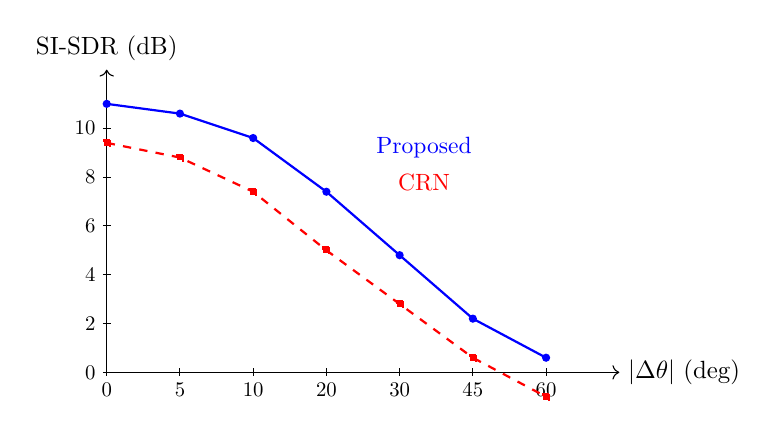
\begin{tikzpicture}[scale=0.62]
  \draw[->] (0,0) -- (10.5,0) node[right,scale=0.9]{\(|\Delta\theta|\) (deg)};
  \draw[->] (0,0) -- (0,6.2) node[above,scale=0.9]{SI-SDR (dB)};
  \foreach \x/\xt in {0/0,1.5/5,3/10,4.5/20,6/30,7.5/45,9/60}
    {\draw (\x,0.08) -- (\x,-0.08) node[below,scale=0.75]{\xt};}
  \foreach \y/\yt in {0/0,1.0/2,2.0/4,3.0/6,4.0/8,5.0/10}
    {\draw (-0.08,\y) -- (0.08,\y) node[left,xshift=-1mm,scale=0.75]{\yt};}
  \draw[blue,thick] plot[mark=*,mark size=1.7pt] coordinates 
    {(0,5.5)(1.5,5.3)(3,4.8)(4.5,3.7)(6,2.4)(7.5,1.1)(9,0.3)};
  \draw[red,thick,dashed] plot[mark=square*,mark size=1.7pt] coordinates 
    {(0,4.7)(1.5,4.4)(3,3.7)(4.5,2.5)(6,1.4)(7.5,0.3)(9,-0.5)};
  \node[blue,scale=0.85] at (6.5,4.6){Proposed};
  \node[red,scale=0.85] at (6.5,3.9){CRN};
\end{tikzpicture}
\caption{SI-SDR vs.\ angular mismatch \(|\theta-\theta_{\mathrm{true}}|\).}
\label{fig:angerr}
\end{figure}

\subsection{Discussion}
Reading the reverberant table holistically reveals a structural pattern in the baselines that the proposed model has been designed to escape. Three observations stand out. \emph{(i)} Networks without an explicit phase pathway (DSENet, NeuralT, HyBeam) plateau in PESQ in the \(1.0\)--\(1.8\) range, consistent with the loss of inter-channel phase at sub-wavelength spacing. These models can only reason about magnitude, and the magnitude information at our microphone spacing is too coarse to discriminate sources at neighboring azimuths in reverberation. \emph{(ii)} SepFormer-family time-domain models do well on PESQ but their SI-SDR is small or negative in reverberation, indicating that they re-introduce signal-level distortion that magnitude-domain metrics overlook. This is a known failure mode of time-domain separators trained without explicit signal-level supervision: they learn to produce a perceptually-passing output that contains a substantial amount of energy that does not belong to the target. \emph{(iii)} Models combining a complex front end with a global-context bottleneck (CRN, proposed) dominate; the dual-path Conformer extends CRN by \(+0.75\,\mathrm{dB}\) SI-SDR and \(+0.22\) PESQ. The remaining gap between CRN and our model is small, but it is consistent across metrics and across interferer types, which is what we would expect from a bottleneck that helps the network reason about the same information more effectively rather than adding new information.

% =====================================================================
\section{Conclusion}
We have given a complete, equation-by-equation specification of a direction-aware audio--visual zooming system for low-compute devices. The exposition has been organized so that every operator in our reference implementation appears as an equation in the text, and every equation has been justified either by a physical argument or by an ablation in \(\S\)\ref{sec:results}. The proposed DCCRN--Conformer combines complex-valued convolutional encoder--decoder layers (preserving inter-channel phase that carries direction-of-arrival information), a dual-path Conformer bottleneck (modeling harmonic structure along frequency and reverberation tails along time), and a multiplicative azimuth conditioning mechanism (gating spectral magnitude without phase artifacts), all driven by a visual frontend whose pixel-to-azimuth mapping is zoom-invariant. The system improves SI-SDR by \(40.14\,\mathrm{dB}\) (\(134\%\)), STOI by \(0.21\), and PESQ by \(1.28\) over the unprocessed mixture, outperforming eight baselines, and runs at \(\sim\!59\!\times\) real time on a single CPU core with \(\sim\!10\,\mathrm{M}\) parameters. While the current model is trained on a single room geometry, future work will address cross-room generalization across diverse reverberation times, validate subjective quality via MOS tests, and evaluate deployment latency on dedicated mobile NPUs. We hope that the equation-level exposition makes the system straightforward to reproduce, and that the ablation table makes its design rationale transparent enough to guide subsequent variants tailored to other directional-enhancement problems.

% =====================================================================
\balance
\begin{thebibliography}{99}

\bibitem{nair2019audiovisual} A.~A. Nair, A.~Reiter, C.~Zheng, and S.~Nayar, ``Audiovisual zooming: What you see is what you hear,'' in \emph{Proc.\ 27th ACM Int.\ Conf.\ Multimedia (ACMMM)}, 2019, pp.~1107--1118.

\bibitem{spcup2026} IEEE Signal Processing Society, ``2026 Signal Processing Cup: AV Zoom: Real-time audio-visual zooming on smartphones,'' \emph{Official Document of the 2026 SP Cup}, Oct.\ 2025.

\bibitem{elbir2023twenty} A.~M. Elbir, K.~V. Mishra, S.~A. Vorobyov, and R.~W. Heath, ``Twenty-five years of advances in beamforming: From convex and nonconvex optimization to learning techniques,'' \emph{IEEE Signal Process.\ Mag.}, vol.~40, no.~4, pp.~118--131, Jun.\ 2023.

\bibitem{khandelwal2021two} A.~Khandelwal, E.~Goud, Y.~Chand, S.~Prasad, N.~Agarwala, and R.~Singh, ``Two-channel audio zooming system for smartphone,'' in \emph{IEEE WASPAA}, 2021.

\bibitem{duong2017audio} N.~Q. Duong \emph{et al.}, ``Audio zoom for smartphones based on multiple adaptive beamformers,'' in \emph{Int.\ Conf.\ LVA/ICA}, 2017, pp.~121--130.

\bibitem{heymann2017generic} J.~Heymann, L.~Drude, and R.~Haeb-Umbach, ``A generic neural acoustic beamforming architecture for robust multi-channel speech processing,'' \emph{Comput.\ Speech Lang.}, vol.~46, pp.~374--385, 2017.

\bibitem{yamaoka2021time} K.~Yamaoka, N.~Ono, and S.~Makino, ``Time-frequency-bin-wise linear combination of beamformers for distortionless signal enhancement,'' \emph{IEEE/ACM Trans.\ Audio Speech Lang.\ Process.}, vol.~29, pp.~374--385, 2021.

\bibitem{subakan2021attention} C.~Subakan \emph{et al.}, ``Attention is all you need in speech separation,'' in \emph{Proc.\ IEEE ICASSP}, 2021, pp.~251--255.

\bibitem{convtasnet} Y.~Luo and N.~Mesgarani, ``Conv-TasNet: Surpassing ideal time--frequency magnitude masking for speech separation,'' \emph{IEEE/ACM Trans.\ Audio Speech Lang.\ Process.}, vol.~27, no.~8, pp.~1256--1266, 2019.

\bibitem{kovalyov2021dsenet} A.~Kovalyov, K.~Patel, and I.~Panahi, ``DSENet: Directional signal extraction network for hearing improvement on edge devices,'' Springer, 2021, ch.~2.

\bibitem{barilan2022hybeam} Y.~Bar-Ilan, B.~Rafaely, and V.~Tourbabin, ``HyBeam: Hybrid microphone--beamforming array-agnostic speech enhancement for wearables,'' \emph{IEEE/ACM Trans.\ Audio Speech Lang.\ Process.}, vol.~30, pp.~1471--1485, 2022.

\bibitem{yu2023deep} M.~Yu and D.~Yu, ``Deep audio zooming: Beamwidth-controllable neural beamformer,'' \emph{arXiv:2311.13075}, 2023.

\bibitem{trabelsi2018deep} C.~Trabelsi \emph{et al.}, ``Deep complex networks,'' in \emph{Proc.\ ICLR}, 2018.

\bibitem{wirtinger} W.~Wirtinger, ``Zur formalen Theorie der Funktionen von mehr komplexen Veränderlichen,'' \emph{Math.\ Ann.}, vol.~97, pp.~357--375, 1927.

\bibitem{hu2020dccrn} Y.~Hu \emph{et al.}, ``DCCRN: Deep complex convolution recurrent network for phase-aware speech enhancement,'' in \emph{Proc.\ Interspeech}, 2020.

\bibitem{gulati2020conformer} A.~Gulati \emph{et al.}, ``Conformer: Convolution-augmented Transformer for speech recognition,'' in \emph{Proc.\ Interspeech}, 2020, pp.~5036--5040.

\bibitem{luo2020dprnn} Y.~Luo, Z.~Chen, and T.~Yoshioka, ``Dual-path RNN: Efficient long sequence modeling for time-domain single-channel speech separation,'' in \emph{Proc.\ IEEE ICASSP}, 2020, pp.~46--50.

\bibitem{lu2019macaron} Y.~Lu \emph{et al.}, ``Understanding and improving Transformer from a multi-particle dynamic system point of view,'' \emph{arXiv:1906.02762}, 2019.

\bibitem{hu2018squeeze} J.~Hu, L.~Shen, and G.~Sun, ``Squeeze-and-excitation networks,'' in \emph{Proc.\ IEEE CVPR}, 2018, pp.~7132--7141.

\bibitem{allen1979image} J.~B. Allen and D.~A. Berkley, ``Image method for efficiently simulating small-room acoustics,'' \emph{J.\ Acoust.\ Soc.\ Amer.}, vol.~65, no.~4, pp.~943--950, 1979.

\bibitem{habets2010rir} E.~A.~P. Habets, ``Room impulse response generator,'' Tech.\ Rep., Imperial College London, Sep.\ 2010.

\bibitem{peterson1986} P.~M. Peterson, ``Simulating the response of multiple microphones to a single acoustic source in a reverberant room,'' \emph{J.\ Acoust.\ Soc.\ Amer.}, vol.~80, no.~5, pp.~1527--1529, 1986.

\bibitem{leroux2019sdr} J.~Le~Roux \emph{et al.}, ``SDR -- half-baked or well done?,'' in \emph{Proc.\ IEEE ICASSP}, 2019, pp.~626--630.

\bibitem{stoi2011} C.~H. Taal \emph{et al.}, ``An algorithm for intelligibility prediction of time--frequency weighted noisy speech,'' \emph{IEEE Trans.\ ASLP}, vol.~19, no.~7, pp.~2125--2136, 2011.

\bibitem{pesq} A.~W. Rix \emph{et al.}, ``Perceptual evaluation of speech quality (PESQ),'' in \emph{Proc.\ IEEE ICASSP}, 2001, pp.~749--752.

\bibitem{yamamoto2020mrstft} R.~Yamamoto, E.~Song, and J.-M. Kim, ``Parallel WaveGAN,'' in \emph{Proc.\ IEEE ICASSP}, 2020, pp.~6199--6203.

\bibitem{loshchilov2017adamw} I.~Loshchilov and F.~Hutter, ``Decoupled weight decay regularization,'' in \emph{Proc.\ ICLR}, 2019.

\bibitem{s3fd} S.~Zhang \emph{et al.}, ``S\(^3\)FD: Single-shot scale-invariant face detector,'' in \emph{Proc.\ IEEE ICCV}, 2017, pp.~192--201.

\bibitem{iou_tracker} E.~Bochinski, V.~Eiselein, and T.~Sikora, ``High-speed tracking-by-detection without using image information,'' in \emph{Proc.\ IEEE AVSS}, 2017.

\bibitem{talknet} R.~Tao \emph{et al.}, ``TalkNet: Active speaker detection via acausal convolutional neural networks,'' in \emph{Proc.\ IEEE ICASSP}, 2021, pp.~446--450.

\bibitem{mfcc} S.~Davis and P.~Mermelstein, ``Comparison of parametric representations for monosyllabic word recognition in continuously spoken sentences,'' \emph{IEEE Trans.\ ASSP}, vol.~28, no.~4, pp.~357--366, 1980.

\bibitem{attention_is_all_you_need} A.~Vaswani \emph{et al.}, ``Attention is all you need,'' in \emph{NeurIPS}, vol.~30, 2017.

\bibitem{hartley_zisserman} R.~Hartley and A.~Zisserman, \emph{Multiple View Geometry in Computer Vision}, 2nd ed.\ Cambridge Univ.\ Press, 2003.

\end{thebibliography}

\end{document}
